\documentclass[10pt, oneside]{article} 
\usepackage{amsmath, amsthm, amssymb, calrsfs, wasysym, verbatim, bbm, color, graphics, geometry, esint, float}
\usepackage{mdframed}



\geometry{tmargin=.75in, bmargin=.75in, lmargin=.75in, rmargin = .75in}  

\newcommand{\bbR}{\mathbb{R}}
\newcommand{\bbC}{\mathbb{C}}
\newcommand{\bbZ}{\mathbb{Z}}
\newcommand{\bbP}{\mathbb{P}}
\newcommand{\bbN}{\mathbb{N}}
\newcommand{\bbQ}{\mathbb{Q}}
\newcommand{\Cdot}{\boldsymbol{\cdot}}
\newcommand{\scA}{\mathscr{A}}
\newcommand{\curl}{\text{curl}}
\newcommand{\Ind}{\text{Ind}}
\newcommand{\Log}{\text{Log}}
\newcommand{\Vol}{\text{Vol}}
\newcommand{\Var}{\text{Var}}
\newcommand{\Cov}{\text{Cov}}
\newcommand{\Corr}{\text{Corr}}
\newcommand{\bbE}{\mathbb{E}}
\newcommand{\bbV}{\mathbb{V}}




\newcommand{\sm}{\setminus}

\theoremstyle{definition}
\newtheorem{exmp}{Example}[section]
\newtheorem{thm}{Theorem}
\newtheorem{defn}{Definition}
\newtheorem{prop}{Proposition}
\newtheorem{conv}{Convention}
\newtheorem{rem}{Remark}
\newtheorem{lem}{Lemma}
\newtheorem{cor}{Corollary}

% Copyright 2021 Paolo Adajar (padajar.com, paoloadajar@mit.edu)
% 
% Permission is hereby granted, free of charge, to any person obtaining a copy of this software and associated documentation files (the "Software"), to deal in the Software without restriction, including without limitation the rights to use, copy, modify, merge, publish, distribute, sublicense, and/or sell copies of the Software, and to permit persons to whom the Software is furnished to do so, subject to the following conditions:
%
% The above copyright notice and this permission notice shall be included in all copies or substantial portions of the Software.
% 
% THE SOFTWARE IS PROVIDED "AS IS", WITHOUT WARRANTY OF ANY KIND, EXPRESS OR IMPLIED, INCLUDING BUT NOT LIMITED TO THE WARRANTIES OF MERCHANTABILITY, FITNESS FOR A PARTICULAR PURPOSE AND NONINFRINGEMENT. IN NO EVENT SHALL THE AUTHORS OR COPYRIGHT HOLDERS BE LIABLE FOR ANY CLAIM, DAMAGES OR OTHER LIABILITY, WHETHER IN AN ACTION OF CONTRACT, TORT OR OTHERWISE, ARISING FROM, OUT OF OR IN CONNECTION WITH THE SOFTWARE OR THE USE OR OTHER DEALINGS IN THE SOFTWARE.

\usepackage{fullpage}
\usepackage{enumitem}
\usepackage{amsfonts, amssymb, amsmath,amsthm}
\usepackage{mathtools}
\usepackage[pdftex, pdfauthor={\name}, pdftitle={\classnum~\assignment}]{hyperref}
\usepackage[dvipsnames]{xcolor}
\usepackage{bbm}
\usepackage{graphicx}
\usepackage{mathrsfs}
\usepackage{pdfpages}
\usepackage{tabularx}
\usepackage{pdflscape}
\usepackage{makecell}
\usepackage{booktabs}
\usepackage{natbib}
\usepackage{caption}
\usepackage{subcaption}
\usepackage{physics}
\usepackage[many]{tcolorbox}
\usepackage{version}
\usepackage{ifthen}
\usepackage{cancel}
\usepackage{listings}
\usepackage{courier}

\usepackage{tikz}
\usepackage{istgame}

\hypersetup{
	colorlinks=true,
	linkcolor=blue,
	filecolor=magenta,
	urlcolor=blue,
}

\setlength{\parindent}{0mm}
\setlength{\parskip}{2mm}

\setlist[enumerate]{label=({\alph*})}
\setlist[enumerate, 2]{label=({\roman*})}

\allowdisplaybreaks[1]

\newcommand{\psetheader}{
	\ifthenelse{\isundefined{\collaborators}}{
		\begin{center}
			{\setlength{\parindent}{0cm} \setlength{\parskip}{0mm}
				
				{\textbf{\classnum~\semester:~\assignment} \hfill \name}
				
				\subject \hfill \href{mailto:\email}{\tt \email}
				
				Instructor(s):~\instructors \hfill Due Date:~\duedate	
				
				\hrulefill}
		\end{center}
	}{
		\begin{center}
			{\setlength{\parindent}{0cm} \setlength{\parskip}{0mm}
				
				{\textbf{\classnum~\semester:~\assignment} \hfill \name\footnote{Collaborator(s): \collaborators}}
				
				\subject \hfill \href{mailto:\email}{\tt \email}
				
				Instructor(s):~\instructors \hfill Due Date:~\duedate	
				
				\hrulefill}
		\end{center}
	}
}

\renewcommand{\thepage}{\classnum~\assignment \hfill \arabic{page}}
\newcommand{\uconv}{\overset{}{\rightrightarrows}}
\makeatletter
\def\points{\@ifnextchar[{\@with}{\@without}}
\def\@with[#1]#2{{\ifthenelse{\equal{#2}{1}}{{[1 point, #1]}}{{[#2 points, #1]}}}}
\def\@without#1{\ifthenelse{\equal{#1}{1}}{{[1 point]}}{{[#1 points]}}}
\makeatother

\newtheoremstyle{theorem-custom}%
{}{}%
{}{}%
{\itshape}{.}%
{ }%
{\thmname{#1}\thmnumber{ #2}\thmnote{ (#3)}}

\theoremstyle{theorem-custom}

\newtheorem{theorem}{Theorem}
\newtheorem{lemma}[theorem]{Lemma}
\newtheorem{example}[theorem]{Example}

\newenvironment{problem}[1]{\color{black} #1}{}

\newenvironment{solution}{%
	\leavevmode\begin{tcolorbox}[breakable, colback=green!5!white,colframe=green!75!black, enhanced jigsaw] \proof[\scshape Solution:] \setlength{\parskip}{2mm}%
	}{\renewcommand{\qedsymbol}{$\heartsuit$} \endproof \end{tcolorbox}}

\newenvironment{reflection}{\begin{tcolorbox}[breakable, colback=black!8!white,colframe=black!60!white, enhanced jigsaw, parbox = false]\textsc{Reflections:}}{\end{tcolorbox}}

\newcommand{\qedh}{\renewcommand{\qedsymbol}{$\blacksquare$}\qedhere}

\definecolor{mygreen}{rgb}{0,0.6,0}
\definecolor{mygray}{rgb}{0.5,0.5,0.5}
\definecolor{mymauve}{rgb}{0.58,0,0.82}

% from https://github.com/satejsoman/stata-lstlisting
% language definition
\lstdefinelanguage{Stata}{
	% System commands
	morekeywords=[1]{regress, reg, summarize, sum, display, di, generate, gen, bysort, use, import, delimited, predict, quietly, probit, margins, test},
	% Reserved words
	morekeywords=[2]{aggregate, array, boolean, break, byte, case, catch, class, colvector, complex, const, continue, default, delegate, delete, do, double, else, eltypedef, end, enum, explicit, export, external, float, for, friend, function, global, goto, if, inline, int, local, long, mata, matrix, namespace, new, numeric, NULL, operator, orgtypedef, pointer, polymorphic, pragma, private, protected, public, quad, real, return, rowvector, scalar, short, signed, static, strL, string, struct, super, switch, template, this, throw, transmorphic, try, typedef, typename, union, unsigned, using, vector, version, virtual, void, volatile, while,},
	% Keywords
	morekeywords=[3]{forvalues, foreach, set},
	% Date and time functions
	morekeywords=[4]{bofd, Cdhms, Chms, Clock, clock, Cmdyhms, Cofc, cofC, Cofd, cofd, daily, date, day, dhms, dofb, dofC, dofc, dofh, dofm, dofq, dofw, dofy, dow, doy, halfyear, halfyearly, hh, hhC, hms, hofd, hours, mdy, mdyhms, minutes, mm, mmC, mofd, month, monthly, msofhours, msofminutes, msofseconds, qofd, quarter, quarterly, seconds, ss, ssC, tC, tc, td, th, tm, tq, tw, week, weekly, wofd, year, yearly, yh, ym, yofd, yq, yw,},
	% Mathematical functions
	morekeywords=[5]{abs, ceil, cloglog, comb, digamma, exp, expm1, floor, int, invcloglog, invlogit, ln, ln1m, ln, ln1p, ln, lnfactorial, lngamma, log, log10, log1m, log1p, logit, max, min, mod, reldif, round, sign, sqrt, sum, trigamma, trunc,},
	% Matrix functions
	morekeywords=[6]{cholesky, coleqnumb, colnfreeparms, colnumb, colsof, corr, det, diag, diag0cnt, el, get, hadamard, I, inv, invsym, issymmetric, J, matmissing, matuniform, mreldif, nullmat, roweqnumb, rownfreeparms, rownumb, rowsof, sweep, trace, vec, vecdiag, },
	% Programming functions
	morekeywords=[7]{autocode, byteorder, c, _caller, chop, abs, clip, cond, e, fileexists, fileread, filereaderror, filewrite, float, fmtwidth, has_eprop, inlist, inrange, irecode, matrix, maxbyte, maxdouble, maxfloat, maxint, maxlong, mi, minbyte, mindouble, minfloat, minint, minlong, missing, r, recode, replay, return, s, scalar, smallestdouble,},
	% Random-number functions
	morekeywords=[8]{rbeta, rbinomial, rcauchy, rchi2, rexponential, rgamma, rhypergeometric, rigaussian, rlaplace, rlogistic, rnbinomial, rnormal, rpoisson, rt, runiform, runiformint, rweibull, rweibullph,},
	% Selecting time-span functions
	morekeywords=[9]{tin, twithin,},
	% Statistical functions
	morekeywords=[10]{betaden, binomial, binomialp, binomialtail, binormal, cauchy, cauchyden, cauchytail, chi2, chi2den, chi2tail, dgammapda, dgammapdada, dgammapdadx, dgammapdx, dgammapdxdx, dunnettprob, exponential, exponentialden, exponentialtail, F, Fden, Ftail, gammaden, gammap, gammaptail, hypergeometric, hypergeometricp, ibeta, ibetatail, igaussian, igaussianden, igaussiantail, invbinomial, invbinomialtail, invcauchy, invcauchytail, invchi2, invchi2tail, invdunnettprob, invexponential, invexponentialtail, invF, invFtail, invgammap, invgammaptail, invibeta, invibetatail, invigaussian, invigaussiantail, invlaplace, invlaplacetail, invlogistic, invlogistictail, invnbinomial, invnbinomialtail, invnchi2, invnF, invnFtail, invnibeta, invnormal, invnt, invnttail, invpoisson, invpoissontail, invt, invttail, invtukeyprob, invweibull, invweibullph, invweibullphtail, invweibulltail, laplace, laplaceden, laplacetail, lncauchyden, lnigammaden, lnigaussianden, lniwishartden, lnlaplaceden, lnmvnormalden, lnnormal, lnnormalden, lnwishartden, logistic, logisticden, logistictail, nbetaden, nbinomial, nbinomialp, nbinomialtail, nchi2, nchi2den, nchi2tail, nF, nFden, nFtail, nibeta, normal, normalden, npnchi2, npnF, npnt, nt, ntden, nttail, poisson, poissonp, poissontail, t, tden, ttail, tukeyprob, weibull, weibullden, weibullph, weibullphden, weibullphtail, weibulltail,},
	% String functions 
	morekeywords=[11]{abbrev, char, collatorlocale, collatorversion, indexnot, plural, plural, real, regexm, regexr, regexs, soundex, soundex_nara, strcat, strdup, string, strofreal, string, strofreal, stritrim, strlen, strlower, strltrim, strmatch, strofreal, strofreal, strpos, strproper, strreverse, strrpos, strrtrim, strtoname, strtrim, strupper, subinstr, subinword, substr, tobytes, uchar, udstrlen, udsubstr, uisdigit, uisletter, ustrcompare, ustrcompareex, ustrfix, ustrfrom, ustrinvalidcnt, ustrleft, ustrlen, ustrlower, ustrltrim, ustrnormalize, ustrpos, ustrregexm, ustrregexra, ustrregexrf, ustrregexs, ustrreverse, ustrright, ustrrpos, ustrrtrim, ustrsortkey, ustrsortkeyex, ustrtitle, ustrto, ustrtohex, ustrtoname, ustrtrim, ustrunescape, ustrupper, ustrword, ustrwordcount, usubinstr, usubstr, word, wordbreaklocale, worcount,},
	% Trig functions
	morekeywords=[12]{acos, acosh, asin, asinh, atan, atanh, cos, cosh, sin, sinh, tan, tanh,},
	morecomment=[l]{//},
	% morecomment=[l]{*},  // `*` maybe used as multiply operator. So use `//` as line comment.
	morecomment=[s]{/*}{*/},
	% The following is used by macros, like `lags'.
	morestring=[b]{`}{'},
	% morestring=[d]{'},
	morestring=[b]",
	morestring=[d]",
	% morestring=[d]{\\`},
	% morestring=[b]{'},
	sensitive=true,
}

\lstset{ 
	backgroundcolor=\color{white},   % choose the background color; you must add \usepackage{color} or \usepackage{xcolor}; should come as last argument
	basicstyle=\footnotesize\ttfamily,        % the size of the fonts that are used for the code
	breakatwhitespace=false,         % sets if automatic breaks should only happen at whitespace
	breaklines=true,                 % sets automatic line breaking
	captionpos=b,                    % sets the caption-position to bottom
	commentstyle=\color{mygreen},    % comment style
	deletekeywords={...},            % if you want to delete keywords from the given language
	escapeinside={\%*}{*)},          % if you want to add LaTeX within your code
	extendedchars=true,              % lets you use non-ASCII characters; for 8-bits encodings only, does not work with UTF-8
	firstnumber=0,                % start line enumeration with line 1000
	frame=single,	                   % adds a frame around the code
	keepspaces=true,                 % keeps spaces in text, useful for keeping indentation of code (possibly needs columns=flexible)
	keywordstyle=\color{blue},       % keyword style
	language=Octave,                 % the language of the code
	morekeywords={*,...},            % if you want to add more keywords to the set
	numbers=left,                    % where to put the line-numbers; possible values are (none, left, right)
	numbersep=5pt,                   % how far the line-numbers are from the code
	numberstyle=\tiny\color{mygray}, % the style that is used for the line-numbers
	rulecolor=\color{black},         % if not set, the frame-color may be changed on line-breaks within not-black text (e.g. comments (green here))
	showspaces=false,                % show spaces everywhere adding particular underscores; it overrides 'showstringspaces'
	showstringspaces=false,          % underline spaces within strings only
	showtabs=false,                  % show tabs within strings adding particular underscores
	stepnumber=2,                    % the step between two line-numbers. If it's 1, each line will be numbered
	stringstyle=\color{mymauve},     % string literal style
	tabsize=2,	                   % sets default tabsize to 2 spaces
%	title=\lstname,                   % show the filename of files included with \lstinputlisting; also try caption instead of title
	xleftmargin=0.25cm
}



\title{UChicago Econometrics Notes: 20510}
\author{Notes by Agustín Esteva, Lectures by Murilo Ramos}
\date{Academic Year 2024-2025}

\begin{document}

\maketitle
\tableofcontents

\vspace{.25in}


\newpage
\section{Lectures}

\subsection{Monday, June 16: Intro to Probability}
\begin{lem}
    (Jensen) Suppose $X$ is a random variable. Let $g: \bbR \to \bbR$ be convex. Then
    \[g(\bbE[X]) \leq \bbE[g(X)]\]
\end{lem}
\begin{proof}
    Since $g$ is convex, then for any $x,y \in \bbR,$ and for any $t\in (0,1)$
    \[g(tx + (1-t)y) \leq tg(x) + (1-t)g(y).\] Let $x = X$ and $y = \bbE[X],$ we see that 
    \[g(tX + (1-t)\bbE[X]) \leq tg(X) + (1-t)g(\bbE[X]).\] Taking expected value,

    \[\bbE[g(tX + (1 - t)\bbE[X]] \leq t\bbE[g(X)] + (1-t)g(\bbE[X])\]
\end{proof}

\begin{defn}
    Let $X$ be a random variable. We say that the \textbf{k\textit{th} moment} of $X$ is $\bbE[X^k].$ We say that the \textbf{k\textit{th} centered moment} of $X$ is $\bbE[(X - \bbE[X])^k].$ We say that the \textbf{k\textit{th} standardized moment} of $X$ is 
    \[\bbE\left[\left(\frac{X - \bbE[X]}{\sqrt{\bbV[X]}}\right)^k\right]\]
\end{defn}

\begin{defn}
    We say that the \textbf{skewness} of $X$ is the third standardized moment of $X.$ We say that the \textbf{kurtosis} of $X$ is the fourth standardized moment of $X.$
\end{defn}

\begin{lemma}
    Let $s \leq t.$ Let $X$ be a positive random variable. If $\bbE[X^t] < \infty,$ then $\bbE[X^s] < \infty.$
\end{lemma}
\begin{proof}
    We can split up $X$ into 
    \[X^t = \mathbbm{1}_{\{X^t \geq 1\}} + \mathbbm{1}_{\{X^t <1\}}.\] It should now be clear that $X^s < X^t + 1$ almost surely. Taking expectations we are done.
\end{proof}

\begin{defn}
    Let $X$ and $Y$ be random variables. We define the \textbf{covariance} of $X$ and $Y$ to be 
    \[\Cov(X,Y) = \bbE[(X - \bbE[X])(Y - \bbE[Y])]\]
\end{defn}



\begin{prop}
    Let $X,Y,Z$ be random variables. Let $a,b,c \in \bbR.$
    \begin{enumerate}
        \item \[\Cov(X,Y) = \Cov(Y,X)\]
        \item \[\Cov(X,Y) = \bbE[XY] - \bbE[X]\bbE[Y]\]
        \[\Cov(X,a) = 0\]
        \item Covariance is bilinear in terms of random variables.
        \item \[\Cov(a + bX, cY) = bc\Cov(X,Y)\]
    \end{enumerate}
\end{prop}

\begin{lemma}
    \[\Var(aX + bY) = a^2\Var(X) + b^2\Var(Y) + 2ab\Cov(X,Y)\]
\end{lemma}
\begin{defn}
    We define the \textbf{correlation} of $X$ and $Y$ to be 
    \[\Corr(X,Y) = \frac{\Cov(X,Y)}{\sqrt{\Var(X)}\sqrt{ \Var(Y)}}\]
\end{defn}
\begin{rem}
    If $\Corr(X,Y)= 0,$ we say that $X$ and $Y$ are uncorrelated, and infer that there is no linear association between $X$ and $Y$. 
\end{rem}

\begin{lemma}
    (C-S Lemma) 
    \[(x,y) \leq \|x\|\|y\|\]
\end{lemma}
\begin{rem}
    Using the $L^2$ norm, we see that 
    \[\bbE[XY] \leq \sqrt{\bbE[X^2]}\sqrt{\bbE[Y^2]}\]
\end{rem}
\begin{proof}
    We prove it for the case of expected value. Let $a\in \bbR.$ Then 
    \begin{align*}
        0 \leq \bbE[(X - aY)^2]= \bbE[X^2] - 2a\bbE[XY] + a^2 \bbE[Y^2]
    \end{align*}
    is a quadratic function with respect to $a.$ Optimizing, 
    \[0 = -2\bbE[XY] + 2a^* \bbE[Y^2]= 0 \implies a^* = \frac{\bbE[XY]}{\bbE[Y^2]}\] Plugging back into (1), 
    \[0 \leq \bbE[X^2] - 2\frac{\bbE[XY]^2}{\bbE[Y^2]} + \frac{\bbE[XY]^2}{\bbE[Y^2]} = \bbE[X^2] - \frac{\bbE[XY]^2}{\bbE[Y^2]}\]
\end{proof}
\begin{rem}
    We see that if $X = aY,$ then by (1), equality in C-S happens. This is an iff.
\end{rem}

\begin{thm}
    For any $X,Y$ random variables, 
    \[|\Corr(X,Y)| \leq 1\] with equality if and only if $Y = a + bX$ almost surely for some $a,b \in \bbR.$
\end{thm}
\begin{proof}
    It suffices to show that $0\leq (\Corr(X,Y))^2 \leq 1.$ But 
    \begin{align*}
        (\Corr(X,Y))^2 &= \frac{\Cov(X,Y)^2}{\Var(X)\Var(Y)}
    \end{align*}
    By definition, it suffices to show that
    \[\Cov(X,Y)^2 = \bbE[(X - \bbE[X])(Y - \bbE[Y])]^2 \leq \bbE[(X - \bbE[X])^2]\bbE[(Y - \bbE[Y])^2]= \Var(X)\Var(Y) \] and so we are done by C-S inequality. Equality comes from equality in C-S.
\end{proof}
\begin{defn}
    Recall that the \textbf{conditional probability} of $X$ given $Y$ is defined to be 
    \[f_{X \mid Y}(x \mid y) = \frac{f_{XY}(x,y)}{f_X(x)}\] The \textbf{conditional expectaion} of $X$ given $Y$ is defined to be 
    \[\bbE[X \mid Y = y] = \int_\bbR x f_{X \mid Y}(x \mid y) = \frac{\int_\bbR x f_{XY}(x,y)}{\int_\bbR  f_Y(y)}\]
\end{defn}

\begin{defn}
    Recall that the \textbf{mean squared error} of $\hat X$ is 
    \[\text{MSE}(\hat{X})= \bbE[(X- \hat X)^2]\]
\end{defn}

\begin{thm}
    $\bbE[Y \mid X]$ is the best predictor for $Y$ given $X$ in an MSE sense. That is, it is the best estimator in the sense that it minimizes the MSE. In other words, 
    \[\bbE[Y \mid X] = \min_{g(X)} \bbE[(Y - g(X))^2]\]
\end{thm}


\begin{thm}
\begin{center}
\fbox{
  \parbox{0.9\textwidth}{
   $\bbE[Y \mid X]$ is the best predictor for $Y$ given $X$ in an MSE sense: That is,  
    \[\bbE[Y \mid X] = \min_{g(X)} \bbE[(Y - g(X))^2]\]
  }
}
\end{center}    
\end{thm}

\begin{prop}
    Let $X,Y,Z$ be random variables, let $g,f$ be functions, and let $a,b \in \bbR$ Then the following hold:
    \begin{enumerate}
        \item $\bbE[g(X) + h(X)Y \mid X] = g(X) + g(X) \bbE[Y \mid X]$
        \item $\bbE[aY = bZ + c \mid X] = a \bbE[Y \mid X] + b \bbE[Z \mid X] + c$
        \item If $Y \leq Z$ almost surely, then $\bbE[Y \mid X] \leq \bbE[Z \mid X]$
        \item  \begin{center}
            
       \fbox{(Tower Law) $\bbE[X] = \bbE[\bbE[X \mid Y]]$} \end{center}
    \end{enumerate}
\end{prop}


\begin{defn}
    We say that $X$ is \textbf{mean independent} of $Y$ if $\bbE[X \mid Y] = c$ almost surely. 
\end{defn}
\begin{rem}
    Note that this notion is not symmetric.
\end{rem}
\begin{lemma}
    If $X$ is mean independent of $Y,$ then
    \begin{itemize}
        \item $\bbE[X \mid Y] = \bbE[X]$
        \item $\bbE[YX] = \bbE[Y]\bbE[X]$
        \item $\Corr(Y,X) = 0$
    \end{itemize}
\end{lemma}
\begin{proof}
Easy!
    \begin{itemize}
        \item $\bbE[X] = \bbE[\bbE[X \mid Y]] = \bbE[c] = c = \bbE[X \mid Y]$
        \item $\bbE[XY] = \bbE[\bbE[XY \mid Y]] = \bbE[Y \bbE[X \mid Y]] = c\bbE[Y] = \bbE[X]\bbE[Y]$
        \item Clear from ii and the fact that $\Cov(X,Y) = \bbE[XY]-\bbE[X]\bbE[Y]$
    \end{itemize}
\end{proof}
\begin{rem}
    Independence implies mean independence implies zero covariance. The converses are in general false. 
    \begin{itemize}
        \item Zero covariance but not mean independent: Let $X$ be a random variable taking values $\{-1, 0, 1\}$ with equal probability:
\begin{align*}
    \Paren{X = -1} &= 1/3 \\
    \Paren{X = 0} &= 1/3 \\
    \Paren{X = 1} &= 1/3
\end{align*}
Let $Y = X^2$.
\item Let $X$ be a random variable taking values $\{-1, 1\}$ with:
\begin{align*}
    \Paren{X = -1} &= 0.5 \\
    \Paren{X = 1} &= 0.5
\end{align*}
Let $Y$ be defined such that:
\begin{itemize}
    \item If $X=1$, $Y$ takes values $\{-1, 1\}$ with $\Paren{Y=-1|X=1}=0.5$ and $\Paren{Y=1|X=1}=0.5$.
    \item If $X=-1$, $Y$ takes values $\{-2, 2\}$ with $\Paren{Y=-2|X=-1}=0.5$ and $\Paren{Y=2|X=-1}=0.5$.
\end{itemize}
    \end{itemize}
\end{rem}

\begin{defn}
    We say that the \textbf{conditional variance} of $Y$ given $X$ is 
    \[\Var(Y \mid X) = \bbE[(Y - \bbE[Y \mid X])^2 \mid X]\]
\end{defn}

\begin{lemma}
    Let $X$ and $Y$ be r.v. and $g,h$ be functions. Then 
    \begin{enumerate}
        \item $\Var(Y \mid X) = \bbE[Y^2 \mid X] - \bbE[Y \mid X]^2$
        \item $\Var(g(X) + h(X) Y \mid X) = \Var(h(X) Y \mid X) = h^2(X)\Var(Y \mid X)$
        \item (Law of Total Variance)
        $\Var(Y) = \bbE[\Var(Y \mid X)] + \Var(\bbE[Y \mid X])$
    \end{enumerate}
\end{lemma}
\begin{proof}
First, 
    \begin{align*}
        \bbE[\Var(Y \mid X)] &= \bbE[\bbE[Y^2 \mid X] - \bbE[Y \mid X]^2]\\
        &= \bbE[\bbE[Y^2 \mid X]] - \bbE[\bbE[Y \mid X]^2]\\
        &= \bbE[Y^2] - \bbE[\bbE[Y \mid X]^2]
    \end{align*}
For the second term,
\begin{align*}
    \Var(\bbE[Y \mid X]) &= \bbE[\bbE[Y \mid X]^2] - \bbE[\bbE[Y \mid X]]^2\\
    &= \bbE[\bbE[Y \mid X]^2] - \bbE[Y]^2\\
\end{align*}
Combining we conclude.
\end{proof}

\newpage
\subsection*{Wednesday, June 18: Intro to Statistics}


We will assume that if we are sampling without replacement with simple random samples, then for a large population, we will treat it as i.i.d. samples. 
\begin{defn}
    Recall that an \textbf{estimator} is a function of the sample such that 
    \[\hat{\theta}_n = \hat{\theta}_n(X_1, \dots, X_n) \]
\end{defn}
\begin{rem}
    Note that an estimator is a random variable, as compared to parameters (e.g, means of populations or variances of populations), which are numbers. 

    The sample mean is a the most frequently used estimator. 

    Recall the analogy principle, where we use $\frac{1}{n}\sum \cdot$ to mim $\bbE[\cdot].$ For example, if $\theta = \Var(X) = \bbE[(X - \bbE(X))^2],$ then 
    \[\hat{\theta}_n = \frac{1}{n} \sum_{i=1}^n (X_i - \overline{X}_n)^2\] As another example, consider 
    \[\theta = \bbP\{X \leq x\} = \bbE[\mathbbm{1}_{X \leq x}]\] then 
    \[\hat{\theta}_n = \frac{1}{n} \sum_{i=1}^n \mathbbm{1}_{X_i \leq x}\]
\end{rem}

\begin{defn}
    Let $\hat{\theta}$ be an estimator for $\theta.$ We define the \textbf{bias} to be 
    \[\text{Bias}(\hat{\theta}) = \bbE[\hat{\theta}] - \theta\]
\end{defn}
\begin{exmp}
    The sample mean is unbiased: 
    \[\bbE[\overline{X}_n] = \bbE[\frac{1}{n}\sum X_i] = \frac{1}{n} \sum \bbE[X_i] = \bbE[X]\]
\end{exmp}
\begin{exmp}
    Consider $\theta = \Var (X)$ with $\hat{\theta} = \frac{1}{n}\sum (X_i - \overline{X}_n)^2.$ Then consider that by the previous example,
    \begin{align*}
        \hat{\theta_n} &= \frac{1}{n}\sum (X_i - \overline{X}_n)^2\\
        &= \frac{1}{n}\sum ((X_i - \bbE[X_i]) - (\overline{X}_n + \bbE[\overline{X}_n]))^2\\
        &= \frac{1}{n}\sum (X_i - \bbE[X_i])^2 - (\overline{X}_n + \bbE[\overline{X}_n])^2\\
        \bbE[\hat{\theta}_n] &= \bbE\left[\frac{1}{n}\sum (X_i - \bbE[X_i])^2 - (\overline{X}_n + \bbE[\overline{X}_n])^2\right]\\
        &= \frac{1}{n}\sum \Var(X_i) - \frac{1}{n}\Var(\overline{X}_n)\\
        &= \Var(X) - \frac{1}{n}\Var(X) = \frac{(n-1)}{n}\Var(X)
    \end{align*}
    Normalize $\frac{n}{n-1}$ to make it unbiased. 

    That is a stupid ass proof. Convince yourself of the following steps:
    \begin{align*}
        \bbE[\hat{\theta}_n] &= \bbE[\frac{1}{n} \sum (X_i - \bar X)^2]\\
        &= \frac{1}{n}\sum \bbE [X_i^2]- \frac{1}{n}\sum \bbE[(\bar X)^2]\\
        &= \bbE[X^2] - \bbE[(\bar X)^2]\\
        &= \Var (X) - \bbE[X]^2 - (\Var(\bar X) - \bbE[\bar X]^2)\\
        &= \Var (X) - \frac{1}{n}\Var(X)\\
        &= \frac{n-1}{n}\Var(X)
    \end{align*}
\end{exmp}

\newpage
\subsection{Final, June 20: Estimator Theory}

\begin{rem}
    Recall that linear combination of normal variables is normal, and thus if $X_1, \dots, X_n \sim N(\mu, \sigma^2),$ then 
    \[\overline{X}_n \sim N(\mu, \frac{\sigma^2}{n}) \implies \frac{\sqrt{n}(\overline{X} - \mu)}{\sigma}\sim N(0,1)\]
\end{rem}
\begin{defn}
    We say that an estimator $\hat{\theta}_n$ \textbf{consistent} if it converges in probability. That is, for any $\epsilon>0,$ 
    \[\lim_{n\to \infty}\bbP\{|\hat{\theta}_n - \theta| >\epsilon\}  = 0\] and we write 
    \[\hat{\theta}_n \xrightarrow[\bbP]{} \theta\]
\end{defn}

\begin{lemma}
    (Chebyshev). If $1\leq p < \infty,$ then for any $\lambda>0,$ we have that 
    \[\bbP\{|X| \geq  \lambda\} \leq \frac{\bbE[|X|^p]}{\lambda^p}\]
\end{lemma}
\begin{proof}
    Letting $A = \{\omega \mid |X| \geq \lambda\},$ we see that 
    \[\bbE[|X|^p] = \int_\Omega |X|^p d\bbP \geq \int_A |X|^p d\bbP \geq \lambda^p \bbP\{A\}\]
\end{proof}

\begin{thm}
\begin{center}
\fbox{
  \parbox{0.9\textwidth}{
    \textbf{Weak Law of Large Numbers.} 
    Let \( X_1, \dots, X_n \sim F \) be i.i.d. Suppose \( \mathbb{E}[X_1^2] < \infty \), then
    \[
    \overline{X}_n \xrightarrow{\bbP} \mathbb{E}[X_1].
    \]
  }
}
\end{center}
\end{thm}


\begin{proof}
    Note that 
    \[\Var(\overline{X}_n) = \bbE[(\overline{X}_n - \bbE[\overline{X}_n])^2] = \bbE[(\overline{X}_n - n\bbE[X_1])^2].\] Hence, 
    \begin{align*}
        \bbP\{|\overline{X}_n - \bbE[X_1]|>\epsilon\} &= \bbP\{(\overline{X}_n - \bbE[X_1])^2 >\epsilon^2\}\\
         &\leq \frac{\Var(\overline{X}_n)}{\epsilon^2}\\
         &= \frac{\Var(X_1)}{n\epsilon^2} \\
         &\to 0
    \end{align*}
    where we use the fact that $\bbE[X_1^2] < \infty$ to say that $\Var(X_1) < \infty.$
\end{proof}



\begin{prop}
    Let $X_1, \dots, X_n \sim F$ be i.i.d. Then $\overline{X}_n$ is consistent.
\end{prop}
\begin{proof}
    As $n\to \infty,$ we know by the law of large numbers that $\overline{X}_n \to \mu$ in probability, and so we are done.
\end{proof}

\begin{thm}
\begin{center}
\fbox{
  \parbox{0.9\textwidth}{
    \textbf{Continuous Mapping Theorem.} \begin{enumerate}
        \item \text{Suppose } $X_n \to x$ in probability and $g$ is continuous. Then 
        \[g(X_n) \xrightarrow[\bbP]{} g(x)\] 
        \item Suppose $X_n \to X$ in distribution and $g$ is continuous. Then 
        \[g(X_n) \xrightarrow[\cal D]{} g(X)\]
    \end{enumerate}}}
\end{center}
\end{thm}

\begin{prop}
        Let $X_1, \dots, X_n \sim F$ be i.i.d. Then 
        \[\hat{\sigma}_x^2 = \frac{1}{n}\sum (X_i - \overline{X})^2\]is consistent.
\end{prop}
\begin{proof}
Note that 
\[\hat{\sigma}_x^2 = \frac{1}{n}\sum(X_i - \overline{X}_n)^2 = \left[\frac{1}{n}\sum X_i^2\right] - (\overline{X}_n)^2 \to \bbE[X^2] - \bbE[X]^2\] by the weak law of large numbers and the continuous mapping theorem using $g(w,x) = w- z^2$ and so we are done. To see the big step, we open up the parenthesis:
\begin{align*}
    \hat{\sigma}_x^2 &= \frac{1}{n}\sum(X_i - \overline{X}_n)^2 \\
    &= \frac{1}{n}\sum X_i^2 - 2X_i\overline{X} + \overline{X}^2\\
    &= \frac{1}{n} X_i^2 - \frac{1}{n}2\overline{X}\sum X_i + \overline{X}^2\\
    &= \frac{1}{n}X_i^2 +\overline{X}^2
\end{align*}
\end{proof}

\begin{exmp}
    Let $(X_1, Y_1), \dots \sim (X,Y)$ be i.i.d with $X,Y \in L^2.$ Let $\theta = \bbE[(X - \mu_X)(Y - \mu_Y)].$ By the anaology principle, 
    \[\hat{\theta}_n = \frac{1}{n}\sum (X_i - \overline{X})(Y_i - \overline{Y})\] Letting $g(w,z,t) = w - zt$ and noting that 
    \[\hat{\theta}_n = \frac{1}{n}\sum X_iY_i - \overline{X}\overline{Y},\] we can use the CMT and the WLLN to show that $\hat{\theta}_n$ is consistent.
\end{exmp}

\begin{defn}
    We say that $X_n$ \textbf{converges in distribution} to $X$ if 
    $F_{X_n} \to F_X(x)$
\end{defn}

\begin{thm}
\begin{center}
\fbox{
  \parbox{0.9\textwidth}{
    \textbf{Central Limit Theorem.}     Let $X_1, \dots, X_n \sim F$ be i.i.d. with mean $\mu$ and $\bbE[X^2] < \infty$ and variance $\sigma^2.$ Then 
    \[\frac{S_n}{\sqrt{n}}\to N(\mu, \sigma^2)\] in distribution
    
    }
    }
\end{center}
\end{thm}


In other words, we have that for large $n,$ 
\[\frac{\sqrt{n}(\bar X - \mu)}{\sigma}\sim N(0,1)\]


\begin{lem}
\begin{center}
\fbox{
  \parbox{0.9\textwidth}{
    \textbf{Slutsky}          Suppose $X_n \to X$ in distribution and $Y_n\to y$ in probability. Then 
    \begin{enumerate}
        \item $X_nY_n \to Xy$ in distribution
        \item $X_n + Y_n \to X + y$ in distribution
        \item $\frac{X_n}{Y_n} \to \frac{X}{y}$ if $y\neq 0$
        \item If $g$ is continuous, then $g(X_n, Y_n)\to g(X, y)$
    \end{enumerate}}}
\end{center}
\end{lem}

\begin{exmp}
    Suppose $X_1, \dots, X_n \sim X$ i.i.d. with $\bbE[X^2] < \infty$ and $\sigma_X^2 >0.$ Recall that the CLT implies that 
    \[\frac{\sqrt{n}(\overline{X}_n - \mu_X)}{\sigma_X} \xrightarrow[d]{} N(0,1).\] In general, we don't observe $\sigma_X^2,$ so we use an estimate $\hat{\sigma}_X^2 \xrightarrow[\bbP]{}\sigma_X^2$ and thus by the CMT 
    \[\hat{\sigma}_X \to \sigma_X.\] Hence, a more feasible statistic for hypothesis tests 
    is 
    \[\frac{\sqrt{n}(\overline{X}_n - \mu_X)}{\hat{\sigma}_X} = \left(\frac{\sqrt{n}(\overline{X}_n - \mu_X)}{\sigma_X}\right)\frac{\sigma_X }{\hat{\sigma}_X} \to N(0,1)\] by Slutsky. 
\end{exmp}

\begin{rem}
\begin{center}
\fbox{
  \parbox{0.9\textwidth}{
    \textbf{Hypothesis Testing}              \begin{enumerate}
        \item (\textit{Step 1}) State $H_0$ and $H_a.$
        \item (\textit{Step 2}) Test statistic and call it 
        \[T_n = g(X_1, \dots, X_n)\] a function of the data.
        \begin{itemize}
            \item $Z$ score could be 
            \[Z = \frac{\sqrt{n}(\overline{X}_n - \mu_X)}{\hat{\sigma}_X}\]
        \end{itemize}
        \item (\textit{Step 3}) Outline rejection region $R$ and critical values. I.e, $\alpha  =0.05$.
        \item (\textit{Step 4}) Conclude (Reject or fail to reject $H_0$)
    \end{enumerate}
    
    }}
\end{center}
\end{rem}


\begin{defn}
    We say that a \textbf{Type I Error} is when the null hypothesis is falsely rejected ($H_0$ is true but it is rejected). We say that a \textbf{Type II Error} is when the failed to be failed to be rejected ($H_0$ is false but it was failed to be rejected)
\end{defn}

\begin{rem}
    The convention is to choose some $\alpha\in \bbR$ such that 
    \[\bbP\{\text{Type I error}\} = \bbP\{T_n \in R \mid H_0\} = \alpha.\] We call $\alpha$ our significance level.
\end{rem}

\begin{exmp}
    (Two sided) Suppose $0 < \Var(X) < \infty$ and $H_0: \bbE[X] =  \mu_0$ and $H_a: \bbE[X] \neq \mu_0$. We let 
    \[T_n = \frac{\sqrt{n}(\overline{X}_n - \mu_0 )}{\hat{\sigma}_X} \xrightarrow[d]{}N(0,1)\] where the convergence happens under the null. We set $\alpha = 0.05,$ and thus 
    \[\bbP\{\left|\frac{\sqrt{n}(\overline{X}_n - \mu_0 )}{\hat{\sigma}_X}\right| \geq c \mid H_0\} = \alpha = 2\left(1 - \Phi(c)\right)  \] by the symmetric of the normal distribution. Solving, 
    \[c = \Phi^{-1}(1 - \frac{\alpha}{2})\]
\end{exmp}

\begin{defn}
    We define the \textbf{$p-$value} to be the smallest $\alpha$ for which we reject $H_0.$
\end{defn}
\begin{exmp}
    $H_0: \bbE[X] \geq 10,$ $H_a: \bbE[X] < 10.$ Found $T_n = -1.5.$ Then the $p-$value is 
    \[\bbP\{Z \leq -1.5\} = p.\] We reject if $p<\alpha$ Suppose now $H_0: \bbE[X] = 10$ and $H_a: \bbE[X]\neq 10.$ Then 
    \[2\bbP\{Z \leq -1.5\} = p.\] More generally, we saw in a $2-$sided test that $c = \Phi^{-1}(1 - \frac{\alpha}{2})$ and we reject if $|T_n| >c,$ and thus reject if
    \[\alpha > 2 (1 - \Phi(|T_n|)) = 2\bbP\{|T_n|\} = p\]
\end{exmp}


\newpage
\subsection{Monday, June 23: Introducing the SLR}


\begin{defn}
    (SLR Model) We say that $y$ is a simple linear regression if 
    \[Y_i = \beta_0 + \beta_1X_i + \sigma U_i,\] where we call $\beta_0$ to be our intercept parameter, $\beta_1$ to be our slope parameter, and $U_i$ is the error term. 
\end{defn}
\begin{rem}
There are three ways to interpret the regressors, and an analysis of these interpretations will yield some insight in why we assume some things:
\begin{enumerate}
    \item (Linear Conditional Expectation)     Suppose that for some $Y$ and $X$ r.v,
    \[\bbE[Y \mid X] = \beta_0 + \beta_1 X.\] We can define 
    \[U = Y - \bbE[Y \mid X].\] Hence, by definition, 
    \[Y = \bbE[Y \mid X] + U = \beta_0 + \beta_1 X + U\] Thus, we see that 
    \[\bbE[U \mid X] = \bbE[Y - \bbE[Y \mid X] \mid X] = 0,\] implying that $U$ is mean independent of $X$ and thus 
    \[\Cov(U,X) = 0\] and moreover, 
    \[\bbE[U] = \bbE[\bbE[U \mid X]] = 0\]
    \item     (Best Linear Predictor (BLP)). Suppose $Y = \beta_0 + \beta_1 X + U = \text{BLP}(Y \mid X) + U$
    \begin{itemize}
        \item Suppose we want to find the best linear predictor for $Y$ as a function of $X$ in the sense that in minimizes $\text{MSE}.$ That is, 
        \[\text{BLP}(Y \mid X) = \min_{(b_0, b_1) \in \bbR^2} \bbE[(Y - b_0 - b_1 X)^2]\] Taking FOC, we find that 
        \[\text{BLP}_1 = (\beta_0, \beta_1)\]
        \item Suppose we want to find the best linear predictor for $\bbE[Y \mid X].$  We want to find 
        \[\text{BLP}_2 = \min_{(b_0, b_1)\in \bbR^2} \bbE[ (\bbE[Y \mid X] - b_0 - b_1 X)^2]\]
    \end{itemize}
    We claim that $\text{BLP}_1 = \text{BLP}_2.$ 
    \begin{proof}
Computing, 
\begin{align*}
    \bbE[(Y - b_0 - b_1 X)^2] &= \bbE[Z^2]\\
    &= \bbE[((Y - \bbE[Y \mid X) + (\bbE[Y \mid X] - b_0 + b_1 X))^2]\\
    &= \bbE[(Y - \bbE[Y \mid X])^2] + \bbE[(\bbE[Y \mid X] - b_0 + b_1 X))^2]
\end{align*}
where we can use orthogonality since 
\begin{align*}
   & \bbE[(Y - \bbE[Y \mid X) (\bbE[Y \mid X] - b_0 + b_1 X)] =\\
    &= \bbE[Y \bbE[Y \mid X]] - \bbE[\bbE[Y \mid X]^2] - b_0\bbE[V] - b_1 \bbE[VX]\\
    &= 0 - 0 - b_1\bbE[\bbE[VX \mid X]] = 0
\end{align*}
Hence, we minimize by taking derivatives and the first term drops out, yielding our result.
    \end{proof}
So we minimized $\bbE[(Y - b_0 - b_1 X)^2] = \bbE[Z^2]$ and to do this explicitly, 
\[\frac{\partial f}{\partial b_0} = -2\bbE[Y - b_0 - b_1 X] \implies \bbE[U] = 0 \qquad \frac{\partial f}{\partial b_1} = -2\bbE[X(Y - b_0 - b_1X)] \implies \bbE[UX] = 0\] Thus, 
\[\bbE[U] = 0\] and 
\[\Cov(U,X) = \bbE[UX] - \bbE[U]\bbE[X] = 0\] and thus the $\text{BLP}$ satisfies the conditions in the previous example.
\item (Causal Interpretation) Suppose our BLP is of the form 
    \[Y = \beta_0 + \beta_1 X + U\] where \textit{we assume} that $\bbE[U] = 0$ and $\Cov(X,U) = \bbE[XU] = 0.$ 
    Then the causal model is of the form
    \[Y = \gamma_0 + \gamma_1 X + V,\] where $V$ is called the causal error (alive!) and can be explained by everything that causes $Y$ which is not encoded in $X$, implying that $\Cov(X,V)\neq 0.$ We define $\gamma_1$ to be 
    \[\frac{\partial Y}{\partial X} \bigg |_{\text{keeping everything constant}} = \gamma_1.\] 

    It is easy to estimate $\beta_0, \beta_1,$ but it is much harder to compute $\gamma_0, \gamma_1.$
\end{enumerate}

\end{rem}


\newpage
\subsection{Wednesday, June 25: SLR Coefficient Theory}
\begin{lem}
    The following equalities hold:
    \begin{enumerate}
        \item \[\sum (X_i - \bar X)(Y_i - \bar Y) = \sum (X_i - \bar X)Y_i\]
        \item \[\sum (X_i - \bar X)^2 = \sum (X_i - \bar X)X_i\]
        \item \[\sum (X_i - \bar X) = 0\]
    \end{enumerate}
\end{lem}

\begin{rem}
\begin{center}
\fbox{
  \parbox{0.9\textwidth}{
    \textbf{SLR Setup in the population}              Let $X,Y,U$ be r.v. such that 
    \[Y = \beta_0 + \beta_1 X + U\] and assume 
    \begin{enumerate}
        \item {$\bbE[U] = 0$}
        \item {$\bbE[XU] = \Cov(X,U) = 0$}
        \item ${0 < \Var(X) < \infty}$
        \item {$(X_1, Y_1), \dots, (X_n, Y_n)\sim (X,Y)$ i.i.d.}
    \end{enumerate}
    
    }}
\end{center}

    From (a), we have that 
    \begin{align*}
        0 &= \bbE[U]\\
        &= \bbE[Y - \beta_0 - \beta_1 X]\\
        &= \bbE[Y] - \beta_0 - \beta_1\bbE[X]
    \end{align*}
    From (b), we have that 
    \begin{align*}
        0 &=\bbE[X(Y - \beta_0 - \beta_1 X)]\\
        &= \bbE[X(Y - \bbE[Y]) - \beta_1(X - \bbE[X])]
    \end{align*} and hence
    \[\bbE[(X - \bbE[X])(Y - \bbE(Y))]=\bbE[X(Y - \bbE[Y])] = \beta_1 \bbE[X(X - \bbE[X])] = \beta_1 \bbE[(X - \bbE[X])(X - \bbE(X))]\]
    Thus, 
    \begin{align}
        \boxed{\beta_1 = \frac{\Cov(X,Y)}{\Var(X)}}
    \end{align}
    \begin{align}
                \boxed{\beta_0 = \bbE[Y] - \frac{\Cov(X,Y)}{\Var(X)}\bbE[X]}
                \end{align}

\end{rem}

\begin{exmp}
        Consider the special case when $X$ is Bernoulli so that $X_1 \sim \text{Bernoulli}(p).$ Note that to compute $\Cov(X,Y) = \bbE[XY] - \bbE[X]\bbE[Y],$ we compute
    \[\bbE[XY] = \bbE[ X\bbE[Y \mid X]]= p \bbE[Y \mid X = 1]\]
    \[\bbE[X]\bbE[Y] = p\bbE[Y] = p\bbE[\bbE[Y \mid X]] = p\left(p\bbE[Y\mid X = 1] + (1-p)\bbE[Y \mid X  =0]\right)\] Thus, we have that 
    \begin{align*}
        \Cov(X,Y) &= p \bbE[Y \mid X = 1] - p^2 \bbE[Y \mid X =1] - p(1-p)\bbE[Y\mid X = 0]\\
        &= p(1-p)\left(\bbE[Y \mid X = 1] - \bbE[Y \mid X = 0]\right)
    \end{align*}
    Hence, 
    \[\beta_1 = \bbE[Y \mid X =1] - \bbE[Y \mid X = 0]\] Computing, we see that 
    \begin{align*}
        \beta_0 &= \bbE[Y] - \beta_1\bbE[X]\\
        &= \bbE[\bbE[Y \mid X]] - \beta_1 p\\
        &= p(\bbE[Y \mid X = 1]) + (1-p)\bbE[Y\mid X = 0] - \left(\bbE[Y \mid X =1] - \bbE[Y \mid X = 0]\right)p\\
        &= \bbE[Y \mid X =0]
    \end{align*}
    Tautological, we have that 
    \[\bbE[Y \mid X] = \bbE[Y \mid X = 0] + \left(\bbE[Y \mid X = 1] - \bbE[Y \mid X = 0]\right)\] implying that by definition, 
    \[\bbE[Y \mid X] = \beta_0 + \beta_1 X.\] 
    \boxed{$Thus, if $X$ is Bernoulli, then$ $\bbE[Y \mid X]$ is linear in $X$ and thus mean independent}.
\end{exmp}

\begin{prop}
\begin{center}
\fbox{
  \parbox{0.9\textwidth}{
    \textbf{SLR Setup in the Sample}              Let $X,Y,U$ be r.v. such that 
    \[Y = \beta_0 + \beta_1 X + U\] and assume 
    \begin{enumerate}
        \item {$\bbE[U] = 0$}
        \item {$\bbE[XU] = \Cov(X,U) = 0$}
        \item ${0 < \Var(X) < \infty}$
        \item {$(X_1, Y_1), \dots, (X_n, Y_n)\sim (X,Y)$ i.i.d.}
    \end{enumerate}
    Then 
    \begin{align}
        \hat \beta_1 &= \frac{\hat\sigma_{XY}}{\hat\sigma_X} = \frac{\sum (X_i - \bar X)(Y_i - \bar Y)}{\sum (X_i - \bar X)^2}
    \end{align}
    \begin{align}
        \hat\beta_2 &= \bar Y - \hat\beta_1 \bar X
    \end{align}
    }}
\end{center}

\end{prop}


\begin{proof}
This is clear using the analogy principle on (1) and (2). 

    For another derivation, recall that 
    \[\bbE[Y - \beta_0 - \beta_1 X] = 0 \qquad \bbE[(Y - \beta_0 - \beta_1 X)X]= 0\] are the first order conditions for $\min_{(b_0, b_1)} \bbE[(Y - b_0 - b_1 X)^2].$ Within the sample, See full derivation in PSET
\end{proof}


\begin{defn}
    Consider a sample regression model such that 
    \[Y_i = \hat{\beta}_0 + \hat{\beta}_1 X_i + \hat{U}_i.\] We call $\hat{U}_i$ the \textbf{residual}, and note that $\hat{\beta}_i$ are both random variables. We define the \textbf{residual} to be 
    \[\hat{U}_i = Y_i - \hat{Y}_i,\] where $\hat{Y}$ is the \textbf{fitted value} such that 
    \[\hat{Y}_i = \hat{\beta}_0 + \hat{\beta}_1 X_i\]
\end{defn}


\begin{rem}
    Recall conditions (a) and (b) in the basic setup. We showed in the above proof the sample equivalents of them for the first order conditions. That is, 
    \begin{align}
    \boxed{\frac{1}{n}\sum \hat{U_i} = 0 }
    \end{align}
    \begin{align}
    \boxed{\frac{1}{n}\sum X_i\hat U_i = 0}
    \end{align}
    Notice that these hold \underline{always} in the OLS, since they are major assumptions. These should not hold in general in causal models.
\end{rem}


\begin{exmp}
    Suppose $Y_i = \hat{\beta}_0 + \hat{\beta}_1 X_i + \hat{U}_i$ where $X_i$ is Bernoulli. Calling $n_0$ the number of times $X_i$ fails and $n_1$ the number of successes, then $n = n_0 + n_1$ is the number in the sample. We call 
    \[\bar Y_0 = \frac{\sum_{i=1}^n Y_i(1 - X_i)}{\sum_{i=1}^n (1 - X_i)} = \frac{1}{n_0} \sum_{i:X_i = 0} Y_i\]
    \[\bar Y_1 = \frac{\sum_{i=1}^n Y_i X_i}{\sum_{i=1}^n X_i} = \frac{\sum_{i : X_i = 1}Y_i}{n_1}\] Thus, we find that (see PSET)
    \[\hat{\beta}_0 = \bar Y_0 \qquad \hat{\beta}_1 = \bar Y_1 - \bar Y_0\]
\end{exmp}

\begin{defn}
    We say that $R^2$ is the \textbf{measure of fit} if it is 
    \[R^2 = \frac{\text{ESS}}{\text{TSS}} = 1 - \frac{\text{SST}}{\text{TSS}}\] where 
    \[\text{Total Sum of Squares (TSS)} = \sum_{i=1}^n (y_i - \bar y)^2\]
    \[\text{Explained Sum of Squares (ESS)} = \sum_{i=1}^n (\hat y_i - \bar y)^2\]
    \[\text{Sum of Squared Residuals (SSR)} = \sum_{i=1}^n \hat{u}_i^2\]
\end{defn}
\begin{prop}
The following hold, 
\begin{enumerate}
    \item \[\text{TSS} = \text{ESS} + \text{SSR}\]
    \item \[R^2 =  1 - \frac{\text{SST}}{\text{TSS}}\]
    \item $R^2 \in [0,1].$
\end{enumerate}
\end{prop}
\begin{proof}
    (a) We compute from the RHS,
    \begin{align*}
        \sum (\hat{y}_i - \bar y)^2  + \sum \hat u_1^2 &= \sum (\hat{y}_i - \bar y)^2  + \sum (y_i- \hat y_i)^2\\
        &= \sum (\hat{y}_i - \bar y - \hat y_i + y_i)^2   - 2\sum (\hat y_i - \bar y)(y_i - \hat y_i)\\
        &= \sum (y_i - \bar y_i)^2 - 2\sum (\hat y_i - \bar y)\hat u_i\\
        &= \sum (y_i - \bar y_i)^2 - 2(\sum \hat y_i u_i - \bar y\sum\hat u_i)\\
        &= \sum (y_i - \bar y_i)^2 - 2(\sum (\beta_0 + \beta_1 x_i) u_i - \bar y\sum\hat u_i)\\
        &= \sum (y_i - \bar y_i)^2\\
        &= \text{TSS}
    \end{align*}
    Where we use Remark 12

    (b) Dividing by TSS in (a), we see that 
    \[1 = R^2 + \frac{\text{SSR}}{\text{TSS}}\]

    (c) From (b), it suffices to see that TSS $\geq$ SSR, but this follows directly from (a)
\end{proof}




\begin{rem}
    Suppose $R^2  = 0,$ then $\text{ESS} = 0$ and $\text{SSR}  = \text{TSS}.$ That is, $\hat{Y}_i = \bar Y.$ Terrible model!!\\

    Suppose $R^2 = 1,$ then $\text{ESS}  = \text{TSS}.$ and $\text{SSR}  =0$ and thus $\hat{u}_i = 0$ and $\hat{y}_i = y_i.$ Goated model.\\

    \underline{$R^2$ does NOT IMPLY CAUSATION.}
\end{rem}

\begin{prop}
\begin{center}
\fbox{
  \parbox{0.9\textwidth}{
    \textbf{(Properties of $\hat\beta$)}              Let $X,Y,U$ be r.v. such that 
    \[Y = \beta_0 + \beta_1 X + U\] and assume 
    \begin{enumerate}
        \item {$\bbE[U] = 0$}
        \item {$\bbE[XU] = \Cov(X,U) = 0$}
        \item ${0 < \Var(X) < \infty}$
        \item {$(X_1, Y_1), \dots, (X_n, Y_n)\sim (X,Y)$ i.i.d.}
    \end{enumerate}
    Then the following hold
    \begin{enumerate}
        \item If $\bbE[U \mid X] = 0$ (alternatively, we have shown that this condition is equivalent to $X$ being binary or to $\bbE[Y \mid X]$ being linear in $X$), then 
        \[\bbE[\hat{\beta_0}] = \beta_0 \qquad \bbE[\hat\beta_1] = \beta_1\]
        \item If $\bbE[X^2] < \infty$ and $\bbE[Y^2] < \infty,$ then 
        \[\hat\beta_0 \xrightarrow[\bbP]{}\beta_0 \qquad \hat\beta_1 \xrightarrow[\bbP]{}\beta_1\]
        \item If $\bbE[X^4] < \infty$ and $\bbE[Y^4] < \infty,$ then 
        \[\sqrt{n}(\hat\beta_1 - \beta_1) \xrightarrow[\cal D]{} N(0, \sigma_1^2)\]
        
    \end{enumerate}
    }}
\end{center}
\end{prop}

\begin{proof}
    \begin{enumerate}
        \item We will first show all these results for $\hat\beta_1.$ Note that 
        \begin{align*}
            \hat\beta_1 &= \frac{\hat\sigma_{XY}}{\hat\sigma_X}\\
            &= \frac{\sum(X_i - \bar X)Y_i}{\sum (X_i - \bar X)^2}\\
            &= \frac{\sum (X_i - \bar X)(\beta_0 + \beta_1 X_i + U_i)}{\sum(X_i - \bar X)^2}\\
            &= \beta_1 + \frac{\sum (X_i - \bar X)U_i}{\hat \sigma_X^2}
        \end{align*}
        We note that 
        \begin{align}
            \hat \beta_1 = \beta_1 + \frac{\sum (X_i - \bar X)U_i}{\sum (X_i - \bar X)^2}
        \end{align}
        Taking $\bbE[\hat\beta_1 \mid X_1, \dots, X_n]$ in (7) and using the assumption that $\bbE[U \mid X] = 0$ and then LIE we conclude. Moreover, 
        \begin{align*}
            \bbE[\hat\beta_0] &= \bbE[\bar Y - \hat\beta_1 \bar X]\\
            &= \bbE[Y] - \beta_1 \bbE[X]\\
            &= \beta_0
        \end{align*}
        \item Under the condition of the second moments, we have showed (Proposition 4 and Example 1.3) that the estimators for covariance and variance are consistent. Thus, using (d) and the CMT for $g(s,t) = \frac{s}{t},$ we see that 
        \[\hat\beta_1 = g(\hat\sigma_{XY}, \hat\sigma_X) \xrightarrow[\bbP]{}g(\sigma_{XY}, \sigma_X) = \beta_1\] Moreover, we use the CMT again with $g(w,s,t) = w - st$ to show that
        \[\hat\beta_0 = g(\bar Y, \hat\beta_1, \bar X) \xrightarrow[\bbP]{} g(\bbE[Y], \beta_1, \bbE[X]) = \beta_0\]
        \item From (7), we see that 
        \begin{align*}
            \sqrt{n}(\hat\beta_1 - \beta_1) &= \frac{\frac{1}{\sqrt{n}}\sum (X_i - \bar X)U_i}{\frac{1}{n}\sum (X_i - \bar X)^2}\\
            &\xrightarrow[\bbP]{} \frac{1}{\sigma_X^2} \left[\frac{1}{\sqrt{n}}\sum (X_i - \bar X)U_i\right]\\
            &=  \frac{1}{\sigma_X^2} \left[\frac{1}{\sqrt{n}}\sum (X_i - \bbE[X] + \bbE[X] - \bar X)U_i\right]\\
            &= \frac{1}{\sigma_X^2}\left[\left(\frac{1}{\sqrt{n}}\sum (X_i - \bbE[X])U_i \right) + \frac{1}{\sqrt{n}} \sum (\bbE[X] - \bar X)U_i\right]\\
            &\xrightarrow[\cal D]{} \frac{1}{\sigma_X^2} N(0, \Var((X - \bbE[X])U))\\
            &= N(0, \frac{1}{(\sigma_X^2)^2}\Var((X - \bbE[X])U))
        \end{align*}
        where we use Slutsky's Lemma for the last convergence, noting that we use the CLT for the first term and the convergence of $\bar X\to \mu_X$ in probability for the second.
    \end{enumerate}
\end{proof}




\newpage
\subsection{Friday, June 27: OVB, Homo/heteroskedasticity, and Inference}
\begin{exmp}
    (Omitted Variable Bias) Causal Model:
\[\text{wages}_i = \gamma_0 + \gamma_1\text{educ}_i + V_i\] where $V_i$ is alive and $\Cov(V_i, X_i) \neq 0.$ 

BLP Model:
\[\text{wages}_i = \beta_0 + \beta_1 \text{educ}_i + U_i\] such that $\Cov(X_i, U_i) = 0.$ Thus, $\gamma_1 \neq \beta_1$ and $\gamma_0 \neq \beta_0.$ 

Does $\beta_1$ over/underestimate $\gamma_1$? Compare to (7), and we see that
\begin{align*}
    \hat\beta_1 &\xrightarrow[\bbP]{} \beta_1\\
    &= \frac{\sigma_{XY}}{\sigma^2_X}\\
    &= \frac{\Cov(X, \gamma_0  + \gamma_1X + V)}{\Var(x)}\\
    &= \frac{\Cov(X, \gamma_0)+ \gamma_1\Cov(X, X) + \Cov(X,V)}{\Var(X)}\\
    &= \gamma_1 + \frac{\Cov(X,V)}{\Var(X)}\\
\end{align*}

\begin{center}
\fbox{
  \parbox{0.9\textwidth}{
    \textbf{(OVB)}              If $\Cov(X,V) >0,$ then $\hat{\beta}_1$ overestimates $\gamma_1.$ If $\Cov(X,V) <0,$ then it underestimates. If $\Cov(X,V) = 0,$ then $\hat{\beta}_1 \to \gamma_1$ in probability.
    }}
\end{center}
\end{exmp}



\begin{rem} In samples, it is often unfeasable to know what $\sigma_1^2$ is. Thus, we often don't use (c) in proposition 7. We estimate using 
\[\hat{\sigma}_1^2 = A\hat\Var(\hat\beta_1)  = \frac{\frac{1}{n}\sum (X_i - \bar X) \hat U_i^2}{(\hat\sigma_X^2)^2}\] and we know that $\hat\sigma_1^2\xrightarrow[\bbP]{} \sigma_1^2.$
\end{rem}


\begin{defn}
    If $U$ is \textbf{homoskedastic}, then $\bbE[U \mid X] = 0$ and $\Var(U \mid X) = \Var(U)$. If $U$ is heteroskedastic, then $\bbE[U  \mid X] = h(X)$
\end{defn}

\begin{prop}
    Suppose $U$ is homoskedastic, then $\sigma_1^2 = \frac{\Var(U)}{\Var(X)}$
\end{prop}

\begin{proof}
    We have that 
\begin{align*}
    \Var((X - \bbE[X])U) &= \bbE[(X - \bbE[X])^2 U^2]\\
    &= \bbE[(X - \bbE[X])^2 \bbE[U^2 \mid X]]\\
    &= \bbE[(X - \bbE[X])^2 \left(\bbE[U^2 \mid X] - \bbE[U \mid X]^2\right)]\\
    &= \bbE[(X - \bbE[X])^2 \Var(U \mid X)]\\
    &= \bbE[(X - \bbE[X])^2 \Var(U)]\\
    &= \Var(U)\Var(X)
\end{align*}
\end{proof}
\begin{exmp}
    (Hetero or Homo?) Suppose $Y$ is Bernoulli($p$) and $\bbE[U \mid X] = 0$ and $Y = \beta_0 +\beta_1 X + U.$ Recall that we have showed that  $\bbE[Y \mid X] = \beta_0 + \beta_1 X.$ First, Note that $Y^2 = Y.$ Next, note that 
    \[\Var(Y \mid X) = \bbE[Y^2 \mid X] - \bbE[Y \mid X]^2 = \bbE[Y \mid X] - \bbE[Y \mid X]^2 = \bbE[Y \mid X][1 - \bbE[Y \mid X]]\] Thus, 
    \[\Var(Y \mid X) = (\beta_0 + \beta_1 X)(1 - \beta_0 - \beta_1 X)\] But we also have that 
    \[\Var(Y \mid X) = \Var(\beta_0 + \beta_1 X +U  \mid X) = \Var(U \mid X)\] which depends on $X,$ and so the error term $U$ is never homoskedastic. 
\end{exmp}

\begin{rem}
(Hypothesis Testing)
    \begin{enumerate}
        \item $H_0: \beta_1 = a$ and $H_1: \beta_1 \neq a$
        \item $T_n = \frac{\hat\beta_1 - \beta_1^{H_0}}{\text{SE}(\hat\beta_1)}$
        \item Same as before
    \end{enumerate}
\end{rem}

\begin{exmp}
    (Hypothesis Test) Test whether $\beta_1 = 1$ or $\beta_1 \neq 1$ at $\alpha 0.05$ We know that 
    \[T = \frac{\hat\beta_1 - \beta_1}{\hat\sigma_1} = \frac{0.6350  -1}{0.0214} = -17.05\] If sample is larger, then $t_\alpha = 1.96$ and we definitely reject.
\end{exmp}

\begin{rem}
(Log Level Regression)
    Recall the Maclaurin expansions:
    \[e^x = 1 + x + \frac{1}{2}x^2 + \cdots \approx 1 + x, \qquad x<<1\]
    \[\log(1+x) = 0 + x + O(x) \approx x, \qquad x<<1.\] Thus, if $Y = \exp\{\beta_0 + \beta_1X + U\},$ then $\Log(Y) \approx \beta_0 + \beta_1 X + U$
    We know that 
    \[\beta_1 = \frac{d\log Y}{dX} = \frac{1}{Y} \frac{dY}{dX} \approx \frac{\Delta Y}{\Delta X}\frac{1}{Y}\] And hence 
    \[\frac{\Delta Y}{Y} \approx \beta_1 \Delta X.\] Thus, 
    \[\boxed{\% \Delta Y \approx 100 \beta_1 \Delta X}\]
\end{rem}

\begin{rem}
    (Log Log Model)
    Suppose $\log(Y) = \beta_0 + \beta_1 \Log(X) + U$ and thus 
    \[\beta_1 = \frac{d\Log Y}{d\Log X} = \frac{1}{Y} \frac{1}{\frac{1}{X}}\frac{dY}{dX}\approx \frac{\% \Delta Y}{\% \Delta X}\] Thus, 
    \[\boxed{\%\Delta Y \approx \beta_1 \%\Delta X}\]
\end{rem}
\begin{rem}
    (Level Log Model) Similarly to before, if 
    $ Y = \beta_0 + \beta_1 \log X + U$, then 
    \[\boxed{\Delta Y \approx \frac{\beta_1}{100}\% \Delta X}\]
\end{rem}


\newpage
\subsection{Monday, June 30: Vector Statistics}






\begin{rem}
    Recall that $A^{-1}$ exists if $\det(A) \neq 0$ or if the columns of $A$ are linearly independent or the rows are. Recall that a vector $\textbf{x} = (x_1, \dots, x_n)^T$ is linearly dependent if there exists scalars $\textbf{c} = (c_1, \dots, c_n)$ such that 
    \[\textbf{c}\textbf{x} = c_1 x_1 + \dots c_n x_n = 0.\]

Suppose $X$ is a random vector such that 
\[X = \begin{pmatrix}x_{11} & x_{12}\\ x_{21} & x_{22}\end{pmatrix}\]
Then $\bbE[X]$ is the expected value of each of its entries. We have that \[\Var(X) = \bbE[(X - \bbE[X])(X - \bbE[X])^T]\] and the covariance matrix is 
\[\begin{bmatrix}
    \Var(X_1) &\Cov(X_1, X_2) & \cdots\\
    \vdots
\end{bmatrix}\] and thus $\Var(X)$ is symmetric. As an example, suppose $X_{n\times 1}$ is a r.v, and $A_{m \times n}$
 is a matrix of constants and $b_{m\times 1}$ is a column, then $\Var(A X + b) = A\Var(X)A^T$
 \end{rem}

\begin{thm}
\begin{center}
\fbox{
  \parbox{0.9\textwidth}{
    \textbf{(The big 4)} Suppose $X_1, \dots, X_n \sim X_{{k \times 1}}$ are i.i.d. Then the following hold, 
    \begin{enumerate}
        \item (\textbf{WLLN}) We have 
        \[\bar X \xrightarrow[\bbP]{}\bbE[X]\]\\
        \item (\textbf{CMT}) Suppose $X_n \xrightarrow[\bbP]{}x$ and $Y_n \xrightarrow[\bbP]{}y,$ and $g$ is continuous then 
        \[g(X_n, Y_n) \xrightarrow[\bbP]{}g(x,y)\]
        \item (\textbf{CLT}) Suppose the second moment of each element in $X$ is finite. Then 
        \[\sqrt{n}(\bar X - \bbE[X])\sim N(0, \Var(X))\]
        \item (\textbf{Slutsky's}) If $X_n \xrightarrow{d}X$ where $X$ is a random matrix and $Y_n \xrightarrow{\bbP} y$ is a constant matrix. Then 
    \begin{enumerate}
        \item $X_nY_N \xrightarrow{d}Xy$ when $Xy$ is defined.
        \item $X_n + Y_n \xrightarrow{d}X + y$ when $X + y$ is defined. 
        \item $X_n Y_n^{-1} \xrightarrow{d} X y^{-1}$ when $Xy$ is defined and $\det(y) \neq 0.$
    \end{enumerate}
    \end{enumerate}
    }}

\end{center}
\end{thm}

\begin{rem}
    If $X_{m\times 1} \sim \mathcal{N}(\bbE[X]_{m\times 1}, \Var(X)_{m\times m})$ then $A X + b$ is also multivariate normal with 
    \[AX  + b \sim \mathcal{N}(A \bbE[X] + b, A \Var(X)A^T)\]
\end{rem}



\begin{thm}
    If $X_{m \times 1} \sim \mathcal{N}(0_{m \times 1}, y_{m\times m})$ and $\det(y)\neq 0.$ Then $g(X, y)= X^T y^{-1} X \sim \chi_{\dim X}^2$. Moreover, suppose $X_n \xrightarrow X_{m\times 1} \sim \mathcal{N}(0, y_{m\times m})$ with $y$ invertible and $y_n \xrightarrow{\bbP} y_{m \times m}.$ Then 
    \[X_n^T y_n^{-1}X_n \xrightarrow{d} X^T y^{-1} X \sim \chi^2_{\dim(X)}\]
\end{thm}
\begin{rem}
    Suppose 
    \[Y = \beta_0 + \beta_1 X_1 + \cdots +\beta_kX_k + U\] Define 
    \[X_{k + 1\times 1} = (1, X_1, \dots, X_k)^T\] and 
    \[\beta_{k + 1 \times  1} = (\beta_0, \beta_1, \dots, \beta_k)^T.\] Then 
    \[Y = X^T \beta + U_{|X|}\]
\end{rem}
\begin{rem}
    \begin{enumerate}
    Again, there are three interpretations for the SLR:
        \item (Linear) Assume $\bbE[Y \mid X] = X^T \beta.$ Define $U = Y - \bbE[Y \mid X] = Y - X^T \beta.$ Then $Y = X^T \beta + U = \bbE[Y \mid X] + U$. Then the $\beta$ are not casual. But then 
        \[\bbE[U \mid X] = \bbE[Y - \bbE[Y \mid X] \mid X] = 0\] and thus $U$ is mean independent of $X.$ Moreover, 
        \[\bbE[X U] = \bbE[\bbE[XU \mid X]] = \bbE[X \bbE[U \mid X]] = 0.\] Note that this is enough (from PSET) to say that 
        \[\bbE[U] = 0.\]
        \item (BLP) The BLP $(Y \mid X)$ is the function that solves 
        \[\min_{b\in \bbR^{k+1}}\bbE[(Y - X^T b)^2]\] which can be shown to be equivalent to 
        \[\min_{b\in \bbR^{k+1}}\bbE[(\bbE[Y \mid X] - X^T b)^2].\] Then, once we find $\text{BLP}(Y \mid X) = X^T\beta,$ we define $U = Y - X^T\beta.$ Rewriting the minimization problem, we have that 
        \[\min_{b \in \bbR^{k+1}} \bbE[(Y - X^T b)^2]\] Taking derivative with respect to $b,$ we see that 
        \[\text{FOC}_b: \qquad -2\bbE[(Y- X^T \beta)X^T] = 0\] applying the transpose and ignoring the $-2,$ we see that (since $Y - X^T\beta$ is a scalar and is therefore its own transpose),
        \[\bbE[X(Y - X^T \beta)^T] = \bbE[X(Y - X^T \beta)] = \bbE[XU]= 0.\] So we get for free that $\bbE[XU] = 0,$ and thus $\bbE[U] = 0$ and $\Cov(X_j,U) = 0$ for any $j \in [k]$.
        \item (Causal Model) Assume 
        \[Y = g(X, U),\] where $X$ are the observed covariates of $Y$ and $U$ are the unobserved covariates. That is, if $g(X,U) = X^T\beta + U,$ then $Y = X^T\beta + U,$ where $\beta_j = \frac{\partial Y}{\partial X_j}$ is the causual effect of $X_j$ on $Y$, holding $X_{-j}$ and $U$ constant. Thus, 
        \[Y = \beta_0 + X_{-0}^T\beta_{-0}+ U = (\beta_0 + \bbE[U]) + X_0^T\beta_{-0} + (U - \bbE[U]) = \beta_0' + X_{-0}^T \beta_{-0} + U'\] Hence, 
        \[\bbE[U'] = 0 \qquad \Cov(X_j, U) \neq 0\]
    \end{enumerate}
\end{rem}


\newpage
\subsection{Monday, July 7: Interactions}
\begin{defn}
    (Notation) We notate
    \[X_{-j} = (1, X_1, \dots, X_{j-1}, X_{j+1}, \dots, X_k)^T\]
\end{defn}
\begin{exmp}
    (Non Linear) 
    Suppose 
    \[Y_i = \beta_0 + \beta_1 X_1 + \beta_2 X_2^2 + \beta_1X_1^3 + \beta_4 X_2 + U_i\]
    Hence, 
    \[\frac{\partial \text{BLP}}{\partial X_1} = \beta_1 + 3\beta_1 \] can be interpreted as the effect of $X_1$ on $Y,$ here $\beta_1$ is the effect when $X _1= 0,$ $\beta_2$ is the sensitivity of the $Y$ with respect to $X_1$ (if positive, then $X_1$ has an increasing effect on $Y$).  
\end{exmp}
\begin{exmp}
    (Interactions) 
    \begin{enumerate}
        \item (Dummy + Cont) Suppose $Y = \beta_0 + \beta_1 X_1 + \beta_2 X_2 + U,$ where $X_1$ is $1$ or $0$ and $X_2$ is a continuum and let's assume a causal model. Then $\beta_1$ is the effect of $X_1$ on $Y$ regardless of $X_2.$ And vice-versa for $\beta_2.$ The problem is that there is no way of measuring the interaction between $X_1$ and $X_2.$ Consider now 
        \[Y = \beta_0 + \beta_1X_1 + \beta_2 X_2 + \beta_3 X_1X_2 + U.\] Suppose $X_1 = 0,$ then $Y = \beta_0' + \beta_2' X_2 + u.$ If $X_1 = 1,$ then $Y = (\beta_0 + \beta_1) + (\beta_2 + \beta_3)X_2 + U,$ which is great because this shows there is a different intercept $(\beta_0 + \beta_1)$ and slope $(\beta_2 + \beta_3)$ for different $X_1.$ This is able to capture the interaction much better. 
        \item (Cont + Cont) Suppose $Y = \beta_0 + \beta_1X_1 + \beta_2 X_2 + \beta_3 X_1X_2 + U.$ Then 
        \[\frac{\partial\text{BLP}}{\partial X_1} = \beta_1 + \beta_3 X_2\] Then $\beta_3$ is the sensitivity of $X_1$ on $Y$ with respect to $X_2.$
        \item (Dummy + Dummy/Difference in Differences) Suppose 
        \[Y = \beta_0 + \beta_1 X_1 + \beta_2 X_2 + \beta_3 X_1 X_2 + U,\] where both $X_1$ and $X_2$ are binary

\begin{table}[H]
    \centering
    \begin{tabular}{cccl}
       $X_1/X_2$&$0$& $1$ &Diff\\
         $0$&  $\beta_0$&  $\beta_0  + \beta_2$&$\beta_2$\\
         $1$&  $\beta_0 + \beta_1$&  $\beta_0 + \beta_1+ \beta_2 + \beta_3$&$\beta_2 + \beta_3$\\
 Diff& $\beta_1$& $\beta_1 + \beta_3 $&$\beta_3$\\
    \end{tabular}
    \caption{Interactions between Dummies}
    \label{tab:my_label}
\end{table}

$\beta_3$ is known as the difference between differences coefficient.
    \end{enumerate}
\end{exmp}


\begin{defn}
    We say that $X_{k+1 \times 1}$ is \textbf{perfectly colinear} if there exists some $\textbf{c} = (c_1, \dots, c_{k+1})^T \neq \textbf{0}$ such that 
    \[\textbf{c}X = 0\]
\end{defn}
\begin{lem}
    Suppose $X$ is not perfectly colinear, then $\bbE[XX^T]$ is invertible. 
\end{lem}
\begin{proof}
    Suppose not. Then there exists some $\textbf{c}\neq 0 $ such that 
    \begin{align*}
        0 &= \bbE[XX^T]\textbf{c}\\
        &= \textbf{c}^T \bbE[XX^T]\textbf{c}\\
        &= \bbE[\textbf{c}^T XX^T\textbf{c}]\\
        &= \bbE[(\textbf{c}X)^2]
    \end{align*} Implying that $\textbf{c}X= 0$ and thus $X$ is perfectly colinear, a contradiction.
\end{proof}

\begin{rem}
    Let $X_1, X_2$ be binary. Then if $X$ contains $X_1$ and $X_2,$ then $X$ is perfectly colinear, as $0 = 1-(X_1 + X_2)$.     If $X_1$ and $X_2$ are colinear. DO NOT build a regressionn with 
    \[Y = \beta_0 + \beta_1 X_1 + \beta_2 X_2 + U\], instead do difference in means 
    \[Y = \beta_0 + \beta_1 X_2 + U\] where $\beta_0$ and $\beta_1$ are the difference in means
    
    or do 
    \[Y = \beta_1 X_1 + \beta_2 X_2 + U\]
\end{rem}




\newpage
\subsection{Wednesday, July 9: $\beta$ Theory}
\begin{thm}
\begin{center}
\fbox{
  \parbox{0.9\textwidth}{
    \textbf{(Deriving $\beta$)} let $Y_{1\times 1}, X_{k +1\times 1 }, U_{k+1\times 1}$ be R.V.s with $Y = X^T \beta + U$ such that
    \begin{enumerate}
        \item $\bbE[XU] = 0$ (which implies $\bbE[U] = 0, \Cov(X_j, U) = 0$). 
        \item No perfect co-linearity in $X.$ 
        \item $\bbE[XX^T] < \infty$ (which implies $\bbE[X_j^2] < \infty$ and $\bbE[X_jX_s] < \infty$)
    \end{enumerate}
    Let $(Y^1, (X^1)^T), \dots, (Y^n, (X^n)^T)\sim (Y, X^T)$ i.i.d. Then 
    \begin{align}
\beta = \bbE[XX^T]^{-1}\bbE[XY]        
    \end{align}
    
    }}
\end{center}

\end{thm}
\begin{proof}
    From (a), we see that 
    \begin{align*}
        0 &= \bbE[XU]\\
        &= \bbE[X(Y - X^T\beta)]\\
        &= \bbE[XY] - \bbE[XX^T]\beta
    \end{align*}
    Rearranging, we see that $\bbE[XX^T]\beta = \bbE[XY],$ and thus we use Lemma 4 to conclude.
\end{proof}

\begin{thm}
\begin{center}
\fbox{
  \parbox{0.9\textwidth}{
    (\textbf{Frisch-Waugh-Lovell}) With the same assumption as in Theorem 9, define 
    \begin{enumerate}
        \item $Y^* := Y - \text{BLP}(Y \mid X_{-j})$
        \item $X_j^* := X_j - \text{BLP}(X_j \mid X_{-j})$
    \end{enumerate} If
    \[Y^* = \beta_0^* + \beta_j^*X_j^* + U^*,\] then $\beta_j^*=  \beta_j$
    
    }}
\end{center}

\end{thm}


\begin{proof}
    From the PSET,
    \begin{itemize}
        \item  $\Cov(X_j^*, X_\ell) = 0$ for all $\ell \neq j$. 
        \item $\Cov(X_j^*, X_j) = \Var(X_j^*)$ (decompose $X_j$ with BLP)
        \item $\Cov(X_j^*, U) = 0$ open up $X_j^*$
    \end{itemize}
    Denoting $\text{BLP}(X_j \mid X_{-j}) = \alpha_0 + \alpha_1 X_1 + \cdots + \alpha_{j-1}X_{j-1} + \alpha_{j+1}X_{j+1} + \cdots + \alpha_k X_k.$ Then computing,
    \begin{align*}
      \beta_j^* &= \frac{\Cov(X_j^*, Y^*)}{\Var(X_j^*)} \\
      &= \frac{\Cov(X_j^*, Y) - \Cov(X_j^*, \text{BLP}(Y \mid X_{-j}))}{\Var(X_j^*)}\\
      &= \frac{\Cov(X_j^*, Y)}{\Var(X_j^*)}\qquad \qquad \qquad \qquad\qquad\text{by (a)}\\
      &= \frac{\Cov(X_j^*, \beta_jX_j + X_{-j}^T \beta_{-j} + U)}{\Var(X_j^*)}\\
      &= \frac{\beta_j \Cov(X_j^*, X_j) + \Cov(X_j^*, X_{-j}^T \beta_{-j}) + \Cov(X_j^*, U)}{\Var(X_j^*)}\\
      &= \beta_j
    \end{align*}
    
\end{proof}
\begin{rem}
    By the FWL thm, we interpret $\beta_j$ as the $\text{BLP}(Y \mid X)$ as partial statistical association between $X_j$ and $Y,$ controlling for $X_{-j}.$ We loosely call this partial correlation:
    \[Z_y = \frac{Y - \mu_y}{\sigma_Y}, \quad Z_{X_j} = \frac{X_j - \mu_{X_j}}{\sigma_{{X_j}}},\] and 
    \[Z-y= \beta_1 Z_{X_1} + \cdots + \beta_k Z_{X_k} + U,\] where $\beta_1$ is the partial correlation between $X_1$ and $Y.$\\

    Moreover, FWL \underline{also works in the sample}. That is, definiting all equal to the above but in the sample, 
    \[\hat\beta_j^* = \hat\beta_j\]
\end{rem}

\begin{thm}
\begin{center}
\fbox{
  \parbox{0.9\textwidth}{
    (\textbf{Estimating $\beta$}) With the assumptions of Theorem 9, the OLS estimator of $\beta$ is given by 
    \begin{align}
        \hat\beta = \left(\frac{1}{n}\sum X^i (X^i)^T\right)^{-1} \left(\frac{1}{n}\sum X^i Y^i\right)
    \end{align}
    }}
\end{center}

\end{thm}
\begin{proof}
    We seek 
    \[\min_{b \in \bbR^{k+1}}\frac{1}{n}\sum (Y^i - (X^i)^Tb)^2 = 0.\] Taking derivative, we see that the first order conditions imply 
    \begin{align*}
        (0)^T &= \left(\sum  (Y^i - (X^i)^T\beta)(X^i)^T\right)^T\\
        &= \sum X^i(Y^i - (X^i)^T\beta)\\
        &= \sum X^i Y^i - \beta\sum X^i(X^i)^T
    \end{align*}
    Rearranging we get the result.  
\end{proof}


\begin{rem}
    In the step when we apply the transpose, we can see that 

\begin{align}
    \frac{1}{n} \sum X^i \hat{U}^i = 0
\end{align}
     which are the mechanical equations of the OLS. This of course implies that 
\begin{align}
    \frac{1}{n} \sum \hat U^i = 0
\end{align}
This is similar to how $\bbE[XU] = \bbE[U] = 0.$
\end{rem}

\begin{defn}
    We say that the \textbf{fitted/predicted} value is 
    \[\hat Y^i := (X^i)^T \hat\beta.\]  We define the \textbf{residual} is 
    \[\hat U^i := Y^i - \hat Y^i = Y^i - (X^i)^T \hat\beta\]
\end{defn}
\begin{rem}
    We still define 
    \[R^2 = \frac{\text{ESS}}{\text{TSS}} = 1 - \frac{SSR}{TSS}\] with $R^2 \in (0,1).$ However, we claim that $R^2$ never decreases with the inclusion of a new regressor. That is, $\text{SSR}$ never increases with this inclusion. Thus, we motivate the definition of the \textbf{adjusted $R^2$} 
    \[\overline{R}^2 := 1- \frac{(n-1)}{(n-k-1)} \frac{\text{SSR}}{\text{TSS}}\]
\end{rem}



\begin{thm}
\begin{center}
\fbox{
  \parbox{0.9\textwidth}{
    \textbf{(Deriving $\beta$)} let $Y_{1\times 1}, X_{k +1\times 1 }, U_{k+1\times 1}$ be R.V.s with $Y = X^T \beta + U$ such that
    \begin{enumerate}
        \item $\bbE[XU] = 0$ (which implies $\bbE[U] = 0, \Cov(X_j, U) = 0$). 
        \item No perfect co-linearity in $X.$ 
        \item $\bbE[XX^T] < \infty$ (which implies $\bbE[X_j^2] < \infty$ and $\bbE[X_jX_s] < \infty$)
    \end{enumerate}
    Let $(Y^1, (X^1)^T), \dots, (Y^n, (X^n)^T)\sim (Y, X^T)$ i.i.d. The OLS estimator for $\beta$ satisfies the following:
    \begin{enumerate}
        \item (\textbf{Unbiased}) If $\bbE[U \mid X] = 0,$ then \[\bbE[\hat\beta] = \beta\]
        \item (\textbf{Consistent}) If $\bbE[Y_j^2] < \infty$ for all $j = 1,2,\dots, k+1,$ then 
        \[\hat \beta \xrightarrow[\bbP]{}\beta\]
        \item (\textbf{Asymptotic Distribution}) If $\bbE[X_j^4] < \infty$ and $\bbE[Y_j^4] < \infty,$ then 
        \[\sqrt{n}(\hat \beta - \beta) \sim N(0, \Sigma)\] where 
        \[\Sigma = \bbE[XX^T]^{-1}\Var(XU)\bbE[XX^T]^{-1}\]
    \end{enumerate}
    
    }}
\end{center}

\end{thm}

\begin{proof}
    \begin{enumerate}
        \item We have that 
        \begin{align*}
            \hat{\beta} &= \left(\frac{1}{n}\sum X^i (X^i)^T\right)^{-1} \left(\frac{1}{n}\sum X^i Y^i\right)\\
            &= \left(\frac{1}{n}\sum X^i (X^i)^T\right)^{-1} \left(\frac{1}{n}\sum X^i ((X^i)^T\beta + U^i)\right)\\
            &= \beta + \left( \frac{1}{n}\sum X^i(X^i)^T\right)^{-1} \frac{1}{n}\sum X^iU^i
        \end{align*}
        Taking conditional expectation of 
        \begin{align}
            \hat{\beta} = \beta + \left( \frac{1}{n}\sum X^i(X^i)^T\right)^{-1} \frac{1}{n}\sum X^iU^i,
        \end{align} 
        we see that if we use (a) on (12), 
        \[\bbE[\hat \beta \mid X_1, \dots, X_n] = \beta_1 +\left( \frac{1}{n}\sum X^i(X^i)^T\right)^{-1} \frac{1}{n}\sum X^i\bbE[U^i \mid X_1, \dots, X_n]  = \beta_1\] Conclude with LIE.
        \item By the WLLN, we have the convergence of 
        \[\frac{1}{n}\sum X^i (X^i)^T \xrightarrow[\bbP]{}\bbE[XX^T]\]
        \[\frac{1}{n}\sum X^i Y^i \xrightarrow[\bbP]{} \bbE[XY]\] so then using the CMT with $g(A,B) = A^{-1}B$ and Lemma 4, we conclude that 
        \[\hat{\beta} = g(\frac{1}{n}\sum X_i X_i^T, \frac{1}{n}\sum X_i Y_i)\xrightarrow[\bbP]{}g(\bbE[X_iX_i^T], \bbE[X_iY_i])  = \beta\]
        \item From equation (12) we use the WLLN, CLT, CMT, and Slutsky to see that
        \begin{align*}
            \sqrt{n}(\hat \beta - \beta) &=  \left( \frac{1}{n}\sum X^i(X^i)^T\right)^{-1} \frac{1}{\sqrt{n}}\sum X^iU^i\\
            &\xrightarrow[\bbP]{}\bbE[XX^T]^{-1} \frac{1}{\sqrt{n}}\sum X^iU^i\\
            &\xrightarrow[\cal D]{}\bbE[XX^T]^{-1}N(0, \Var(XU))\\
            &= N\left(0, \bbE[XX^T]^{-1}\Var(XU)\bbE[XX^T]^{-1}\right)
        \end{align*}
        Where the last equality is due to $\bbE[XX^T]$ being invertible and thus symmetric. 
    \end{enumerate}
\end{proof}

\begin{rem}
    \textbf{(Omitted Variable Bias)}
    Suppose 
    \[Y = \beta_0 + \beta_1 X_1 + \beta_2 X_2 + U\] satisfies the conditions of Theorem 12 (b). Suppose it is difficult to measure $X_2$ directly, so consider estimating with OLS the new 
    \[Y = \alpha_0+ \alpha_1 X_1  + V.\] We know by Proposition 7 that 
    \begin{align*}
    \hat\alpha_1 \xrightarrow[\bbP]{}\alpha_1 &= \frac{\Cov(X_1,Y)}{\Cov(X_1)}\\
    &= \frac{\Cov(X_1, \beta_0 + \beta_1 X_1 + \beta_2 X_2 + U)}{\Var(X_1)}\\
    &= \beta_1 + \beta_2 \frac{\Cov(X_1, X_2)}{\Cov(X_2)}
    \end{align*}
    \begin{center}
\fbox{
  \parbox{0.9\textwidth}{
    \textbf{(OVB)}   \begin{table}[H]
        \centering
        \begin{tabular}{cccc}
            $$\beta_2$$/($\Cov(X_1, X_2$)& $+$ & $-$ &$0$ \\
            $+$ & $+$ & $-$  & $0$\\
            $-$ &  $-$& $+$ & $0$\\
             $0$&  $0$&  $0$& $0$\\
        \end{tabular}
        \caption{Effects of OVB}
    \end{table}
    }}
\end{center}
\end{rem}

\begin{exmp}
    Suppose a causal MLR of
    \[\text{muscle mass} = \beta_0 + \beta_1 \text{gymtime} + \beta_2 \text{genes} + U\]
    Genes are hard to measure, so we consider estimating the following with OLS
    \[\text{muscle mass}= \alpha_0 + \alpha_1 \text{gymtime} + V.\] By OLS, We require that $\Cov(V, \text{gymtime}) = 0.$  The following step would be to investigate $\beta_2$ and $\Cov(X_1,X_2)$ and use Table 2.
\end{exmp}

\begin{rem}
    (\textbf{Measurement Error})
    \begin{itemize}
        \item A measurement error in $Y$ is benign, and doesn't cause OVB, only increases $\Var(\hat\beta_j)$
        \item Measurement error in $X$ is bad. Common case is classical measurement error (CME). 
        To see this, suppose 
        \[Y = \beta_0 + \beta_1 X + U,\] but a researcher estimates \[Y = \alpha_0 + \alpha_1 X^* + V\] with OLS, where $X^*$ is a ill-measured $X$ with $X^* = X + Z,$ where $\bbE[Z] = \Cov(X,Z) = \Cov(U,Z) = 0.$ We know that 
        \begin{align*}
            \hat \alpha_1 \xrightarrow[\bbP]{}\alpha_1 &= \frac{\Cov(X^*, Y)}{\Cov(X^*)}\\
            &= \frac{\Cov(X + Z, \beta_0 + \beta_1 X + U)}{\Var(X + Z)}\\
            &= \frac{\beta_1\Var(X) + \Cov(X,U) + \beta_1\Cov(Z,X) + \Cov(Z,U)}{\Var(X) + \Var(Z) + 2\Cov(X,Z)}
            \end{align*}
            Using various assumptions, we have derived 
        \begin{center}\fbox{
  \parbox{0.9\textwidth}{
    \textbf{(Attenuation Bias)}   
    \[
\hat{\alpha_1} \xrightarrow[\bbP]{} \beta_1\underbrace{ \frac{\Var(X)}{\Var(X) + \Var(Z)}}_{\text{attenuation bias, $\leq 1$}}
\]
Measurement error always pulls $\hat{\alpha}_1$ towards $0.$ 

    }}
\end{center}
    \end{itemize}
\end{rem}

\begin{prop}
If $U$ is homoskedastic, then 
    \[\Sigma = \bbE[XX^T]^{-1}\Var(U).\]
    \end{prop}
\begin{proof}
Since $U$ is homoskedastic, then $\bbE[U \mid X] = 0$ and $\Var(U \mid X) = \Var(U).$ Hence, 

    \begin{align*}
        \Var(X U)  &= \bbE[XX^T U^2] - \bbE[XU]\bbE[XU]^T\\
        &= \bbE[XX^T \bbE[U^2 \mid X]]\\
        &= \bbE[XX^T \Var(U \mid X)]\\
        &= \bbE[XX^T \Var(U)] \qquad \text{(homosk)}\\
        &= \Var(U)\bbE[X X^T]
    \end{align*}
    Thus, 
    \begin{align*}
        \Sigma &= \bbE[XX^T]^{-1} \Var(U)\bbE[XX^T] \bbE[XX^T]^{-1} = \Var(U)\bbE[XX^T]^{-1}
    \end{align*}
\end{proof}

\begin{rem}
    If  $U$ is not homosk, then using the analogy principle, 
    \begin{align}
\hat \Sigma = \left[\frac{1}{n}\sum X^i (X^i)^T\right]^{-1} \left[\frac{1}{n} \sum  (\hat U^i) ^2 X^i(X^i)^T\right]\left[\frac{1}{n}\sum X^i (X^i)^T\right]^{-1}        
    \end{align}

\end{rem}

\newpage
\subsection{Friday, July 11: Hypothesis Testing}

\begin{lem}
    Suppose $X_n \xrightarrow[\cal D]{}N(0, y_n)$ and $y_n \xrightarrow[\bbP]{}y.$ Then 
    \[X_n ^Ty^{-1}X_n \xrightarrow[\cal D]{}X^Ty^{-1}X \sim \chi_{\dim (X)}^2\]
\end{lem}

\begin{rem}
    \textbf{(Hypothesis Testing for Linear Combinations of $\beta$)}
    \begin{enumerate}
        \item[(1)] $H_0: R\beta = r,$ $H_a: R\beta \neq r,$ where, usually $r = \textbf{0}$ and $R$ is the matrix testing the linear combinations. 
        \item[(2)] Since $\sqrt{n}(\hat\beta - \beta) \xrightarrow[\cal D]{} N(0, \Sigma),$ then by Slutsky's Lemma
        \[\sqrt{n}(R \hat\beta - R\beta)\xrightarrow[\cal D]{}N(0, R\Sigma R^T).\] As usual, $\Sigma$ is unattainable, so we use (13) as a consistent estimator. From Lemma 5,
        \begin{center}\fbox{
  \parbox{0.9\textwidth}{
    \textbf{(Wald's Statistic)}   
    \[
T_n = n(R\hat\beta - R\beta)^T (R\hat\Sigma R^T)^{-1} (R\hat\beta - R\beta) \xrightarrow[\cal D]{} \chi_{\dim(R\beta)}^2
\]

    }}
\end{center}
\item [(3)] The usual end for hypothesis testing.
    \end{enumerate}
\end{rem}

\begin{exmp}
    
\end{exmp}



\begin{exmp}
Suppose $Y = \beta_0 + \beta_1 X_1 + \beta_2 + U,$ with 
    \[H_0:\beta_1 + 2\beta_2 = 0 \quad H_a: \beta_1 + 2\beta_2 \neq 0.\] Then 
    \[R = \begin{bmatrix}
        0 & 1 & 2
    \end{bmatrix}\] and $r = \textbf{0}.$
\end{exmp}

    \begin{exmp}
       \[ H_0: \beta_1, \beta_2 = 0 \quad H_a: \beta_1 \neq 0 \cup \beta_2 \neq 0\], then 
       \[R = \begin{bmatrix}
           0 &1 & 0\\
           0 & 0 & 1
       \end{bmatrix} \implies R\beta = \begin{bmatrix}
           \beta_1 \\ \beta_2
       \end{bmatrix}\] Under $H_0,$ $R\beta = r,$ where $r = \begin{bmatrix}
            0 \\ 0
       \end{bmatrix}$. Recall that 
       \[\sqrt{n}(\hat{\beta} - \beta) \to N(0, \Sigma) \implies \sqrt{n}(R\hat{\beta} - R\beta) \to N(0, R \Sigma R^T)\] we can measure the scalar of how far away the data is from the values:
       \[n(R\hat\beta - R\beta)^T(R\sum R^T)^{-1}(R\hat\beta - R\beta)\]
    \end{exmp}

    Let 
    \[T_n = n(R\hat\beta - R\beta^{H_0})^T(R \hat\Sigma R^T)^{-1}(R\hat\beta - R\beta) \xrightarrow[d]{}\chi^2_{\dim (R\beta)}\]



\begin{rem}
(\textbf{F-Statistic Hypothesis Testing})
\underline{Assume $U$ is homoskedastic}., and consider the SLR
\[Y^i = \beta_0 + \beta_1 X_{1}^i + \beta_2 X_{2}^i + U^i \quad (\text{unrestricted model}).\] 
\begin{enumerate}
    \item [(1)] \[H_0: \beta_1, \beta_2 = 0 \qquad H_a: \beta_1 \neq 0\cup \beta_2 \neq 0\]
    \item [(2)] Under $H_0:$ \[Y^i = \beta_0  + U^i \quad (\text{restricted model})\] Compute 
    \[F_n = \frac{\frac{1}{q}\left(\text{SSR}_r - \text{SSR}_{ur}\right)}{ \frac{1}{(n - k_{ur} - 1)}\text{SSR}_{ur}} = \frac{\frac{1}{q}\left(R^2_{ur} - R^2_r\right)}{ \frac{1}{(n - k_{ur} - 1)}(1-R^2_{ur})}, \] where $q$ is the number of constraints, and $K_{ur}$ is the number of regressor in the $ur$ model.
    \item [(3)] $F$ is distrbuted as $F_{q, \,n-K_{ur}- 1}$
\end{enumerate}


\newpage
\subsection{Monday, July 14: Instrument Variables in SLR}
\begin{defn}We say that $X_j$ is \textbf{endogenous} if $\Cov(X_j, U) \neq 0.$ Else, we say that $X_j$ is \textbf{exogenous.}
\end{defn}

Until otherwise stated, we consider 
\[Y = X^T\beta + U,\] where there is at least one endogenous variable. From Remark 22, (c), we note that $\bbE[U] = 0.$ how do we estimate $\beta$ in this scenario?
\begin{rem}
    There are three main sources of endogeneity:
    \begin{enumerate}
        \item OVB (when $U$ is alive, see Example 1.9)
        \item Measurement Error (When $X$ is not quite right, see Remark 28)
        \item Simultaneity Bias (See Example 1.19)
    \end{enumerate}
\end{rem}

\begin{defn}
    Suppose $Y = X^T\beta + U.$ We say that a r.v. $Z$ is an \textbf{instrument} if 
        \begin{itemize}
            \item $\Cov(Z,U) = \bbE[ZU]= 0$ (instrument exogeneity)
            \item $\Cov(X,Z) \neq 0$ (instrument relevance)
        \end{itemize} 
\end{defn}
\begin{exmp}
    (Civil conflict in Africa) Consider 
    \[\text{conflict}_i = \beta_0 + \beta_1 \text{growth}_i + U_i,\] and consider 
    \[Z_i: \text{rainfall} \text{ s.t. } \Cov(X,Z) \neq 0, \Cov(Z,U) = 0\]
\end{exmp}
\hline
\begin{rem}
    (\textbf{Case 1: SLR}) 
\begin{defn}
    Suppose $Y = \beta_0 + \beta_1 X + U.$ We say that a r.v. $Z$ is an \textbf{instrument} if 
        \begin{itemize}
            \item $\Cov(Z,U) = \bbE[ZU]= 0$ (instrument exogeneity)
            \item $\Cov(X,Z) \neq 0$ (instrument relevance)
        \end{itemize} 
\end{defn}    
Suppose $Y= \beta_0 + \beta_1 X + U,$ where $X$ is endogenous. 
    
    We derive
    \begin{align*}
        0 &= \bbE[U]\\
          &= \bbE[Y] - \beta_0 - \beta_1 \bbE[X]
    \end{align*}
    gives us 
    \begin{align}
        \beta_0 = \bbE[Y] - \beta_1 \bbE[X]
    \end{align}
    Plugging in (14)
    \begin{align*}
        0 &= \bbE[ZU]\\
        &= \bbE[Z(Y - \beta_0 - \beta_1 X)]\\
        &= \bbE[Z(Y - \bbE[Y] + \beta_1 \bbE[X] - \beta_1 X)]\\
        &= \bbE[Z(Y - \bbE[Y])] - \beta_1 \bbE[Z(X - \bbE[X])]\\
        &= \Cov(Z,Y) - \beta_1 \Cov(Z,X)
    \end{align*} give us 
    \begin{align}
        \beta_1 &= \frac{\Cov(Z,Y)}{\Cov(Z,X)}
    \end{align}
    Note that when $X$ is binary, this nicely simplifies to 
    \begin{center}\fbox{
  \parbox{0.9\textwidth}{
    \textbf{(Local Average Treatment)}   
    \[
 \beta_1 = \frac{\bbE[Y \mid Z = 1] - \bbE[Y \mid Z = 0]}{\bbE[X \mid Z = 1] - \bbE[X \mid Z = 0]} = \frac{\pi_1}{\alpha_1}
\]

    }}
\end{center}
    
    where $\pi_1$ and $\alpha_1$ are the coefficients from regressing $Y$ and $X$ on $Z,$ respectively. 
\begin{thm}
\begin{center}
\fbox{
  \parbox{0.9\textwidth}{
    \textbf{(Estimation with SLR Instrument Variables)} let $Y,X,U,Z$ be R.V.s with $Y = \beta_0 +  \beta_1X + U$ such that
    \begin{enumerate}
        \item $\bbE[U] = 0$. 
        \item $\bbE[ZU] = 0$ (Exogeneity).
        \item $\Cov(X,Z) \neq 0$
    \end{enumerate}
    Let $(Y^1, X^1, Z^1), \dots, (Y^n, X^n, Z^n)\sim (Y, X, Z)$ i.i.d. Then the IV estimator for $\beta$ given by 
\begin{align}
    \hat\beta_1^{IV} &= \frac{\hat \sigma_{ZY}}{\hat \sigma_{ZX}}\\
    \hat\beta_0^{IV} &= \bar Y - \hat\beta_1^{IV} \bar X
\end{align}
satisfies
    
    \begin{enumerate}
    \item The sample equivalents of (a) and (b):
    \begin{align*}
        0 &= \frac{1}{n} \sum (Y^i - \hat\beta_0^{IV} - \hat \beta_1^{IV} X^i) = \frac{1}{n}\sum \hat U^i\\
        0 &= \frac{1}{n}\sum Z^i(Y^i - \hat\beta_0^{IV} - \hat\beta_1^{IV} X^i) = \frac{1}{n}\sum Z^i \hat U^i
    \end{align*}
        \item (\textbf{Consistent}) If $\bbE[Y^2], \bbE[Z^2], \bbE[X^2] < \infty,$ then both $\hat\beta_0^{IV}$ and $\hat\beta_1^{IV}$ are consistent.
        \item (\textbf{Asymptotic Distribution}) If $\bbE[X^4], \bbE[Y^4], \bbE[Z^4] < \infty$, then 
        \[\sqrt{n}(\hat \beta_1^{IV} - \beta_1) \sim N(0, \sigma_{1,IV}^2)\] where 
        \[\sigma_{1, IV}^2 = \frac{\Var((Z - \bbE[Z])U)}{\Cov^2(X,Z)}\]
    \end{enumerate}
    
    }}
\end{center}

\end{thm}

\begin{proof}
    \begin{enumerate}
        \item From the first equation, we can derive $\hat\beta_0^{IV}.$
        \begin{align*}
            0 &= \frac{1}{n}\sum(Y^i - \hat\beta_0^{IV} - \hat\beta_1^{IV} X^i)\\
            &= \bar Y - \hat\beta_0^{IV} - \hat\beta_1^{IV} \bar X
        \end{align*} Similarly, we plug in (17) into the second equation to see how 
        \begin{align*}
            0 &= \frac{1}{n}\sum Z^i(Y^i - \hat\beta_0^{IV} - \hat\beta_1^{IV} X^i)\\
            &= \frac{1}{n}\sum Z^i(Y^i - (\bar Y - \hat\beta_1^{IV} \bar X) - \hat\beta_1^{IV} X^i)\\
            &= \frac{1}{n}\sum (Y^i - \bar Y)Z^i - \hat\beta_1^{IV} \frac{1}{n}\sum (X^i - \bar X)Z^i
        \end{align*}
        yields the answer.
        \item We know that $\hat\sigma_{YZ} \xrightarrow[\bbP]{}\sigma_{YZ}$ and $\hat \sigma_{XZ}\xrightarrow[\bbP]{}\sigma_{XZ}.$  use continuous mapping theorem to conclude.
        \item We can write
        \begin{align}
            \hat\beta_1 ^{IV}&= \frac{\sum (Z^i  - \bar Z)Y^i}{\sum (Z^i - \bar Z)X^i}=\frac{\sum (Z^i  - \bar Z)(\beta_0 + \beta_1X^i + U^i)}{\sum (Z^i - \bar Z)X^i} = \beta_1  + \frac{\sum(Z^i - \bar Z)U^i}{\sum (Z^i - \bar Z)X^i}
        \end{align}
        From (18) we see that, by using a combination of WLLN, CLT, then WLLN, then Slutsky's Lemma, 
        \begin{align*}
            \sqrt{n}(\hat\beta_1^{IV} - \beta_1) &= \frac{\frac{1}{\sqrt{n}}\sum(Z^i - \bar Z)U^i}{\frac{1}{n}\sum(Z^i - \bar Z)X^i}\\
            &\xrightarrow[\cal \bbP]{} \frac{\frac{1}{\sqrt{n}}\sum(Z^i - \bbE[Z])U^i}{\frac{1}{n}\sum(Z^i - \bbE[Z])X^i + \frac{1}{n}\sum (\bbE[Z] - \bar Z)X^i}\\
            &\xrightarrow[ \bbP]{} \frac{\frac{1}{\sqrt{n}}\sum(Z^i - \bbE[Z])U^i}{\Cov(Z,X)}\\
            &\xrightarrow[\cal D]{}\frac{N(0, \Var((Z - \bbE[Z])U))}{\Cov(Z,X)}
        \end{align*}
        As usual, we usually estimate this variance by 
            \[\hat\sigma_{1, IV}^2 = \frac{\sum (Z_i - \bar Z)\hat U_i}{\sum (Z_i - \bar Z)(X_i - \bar X)}\]
    \end{enumerate}
\end{proof}

\begin{rem}
    (\textbf{Biased}) What happens to the bias? In order to establish unbiasness, it is clear from (18) that we would need $\bbE[U^i \mid X^i, Z^i]= 0.$ But then using the LIE it is clear that $\bbE[X^iU^i] = 0.$ But this then implies that $\Cov(X^i, U^i) = 0,$ a contradiction to $X^i$ being endogenous.
\end{rem}

\begin{exmp}
    (\textbf{Simultaneity Problem})
Let 
                \[Q^d(p) = \beta_0 + \beta_1 p + U^d\]
                \[Q^s(p) = \alpha_0 + \alpha_1 p + \alpha_2 Z + U^s\]
assume $\beta_1 < 0, \alpha_1 >0,$ and $\Cov(U^d, U^s) = 0$ and $Z$ is a supply shifter with $\Cov(Z,U^s) = \Cov(Z,U^d) = 0$ and $\Var(Z)>0.$ Suppose further that $\alpha_2 \neq 0.$ 


Solving for $P$ in $Q(P) = Q(P) = Q$ gives 
\[\frac{1}{\alpha_1 - \beta_1}(\beta_0 - \alpha_0 - \alpha_2 Z + U^d - U^s),\] and hence $P$ is endogenous in both $Q^d(P)$ and $Q^s(P)$ with 
\[\Cov(P,U^d) = \frac{\Var(U^d)}{\alpha_1-\beta_1}>0 ,\qquad \Cov(P,U^d) = \frac{-\Var(U^s)}{\alpha_1-\beta_1} <0\] From OVB analysis, the above imply that (Example 1.9) the BLP coefficients overestimate $\beta_1$ and underestimate $\alpha_1.$\\

It can be worked out that $\Cov(Z,P) \neq 0$ given the assumptions, implying that $Z$ is an instrument variable and we can estimate a consistent estimator!
\end{exmp}
\end{rem}

\hline


\begin{rem}
    (\textbf{Case 2: MLR})    For the following case, we will consider the model $Y = X^T\beta + U,$ where $X_1$ is endogenous and $X_{-1}$ are exogenous and (WLOG) $\bbE[U] = 0.$
\begin{defn}
    Suppose $Y = X^T\beta + U.$ We say t We say that a r.v. $Z$ is an \textbf{instrument} if 
        \begin{itemize}
            \item (instrument exogeneity) $\Cov(Z,U) = \bbE[ZU]= 0$ 
            \item (instrument relevance) Letting $W = (1, Z, W_2, \dots, W_k)$ not be perfectly colinear and $\pi = (\pi_0, \pi_1, \dots, \pi_k)$ such that $\pi_1 \neq 0,$ then 
            \[X_1 = \text{BLP}(X_1 \mid W) + V = W^T\pi\]
        \end{itemize} 
\end{defn}

\begin{prop}
   Suppose $Y = X^T\beta + U$ and $X_1$ is the only endogeneous variable. Then the following are equivalent:
   \begin{enumerate}
       \item $Z$ is relevant;
       \item $\bbE[WX^T]$ is invertible;
       \item $\bbE[WW^T]^{-1}\bbE[WX^T]$ is invertible
   \end{enumerate}
\end{prop}
\begin{proof}
    ($a\iff c$) Suppose $Z$ is relevant. Consider regressing $X$ by $W.$ then the BLP coefficient is given by (see Theorem 9) \[\alpha = \bbE[WW^T]^{-1}\bbE[WY] = \begin{pmatrix}
    1 & \pi_0& 0 &\cdots & 0\\
    0 & \pi_1& 0 &\cdots & 0\\
    0 & \pi_2& 1 & \cdots & 0\\
    \vdots & \vdots & \vdots & \ddots & \vdots\\
    0 & \pi_k & 0 & 0 & 1
\end{pmatrix}\] which is clearly if and only if invertible when $\pi \neq 0.$ 

($c\iff b$) This is a result from linear algebra. More generally, if $A$ is an invertible matrix, then $B$ is invertible if and only if $A^{-1}B$ is invertible. For the forward direction we see that since $A$ and $B$ are invertible, then $B^{-1}A$ is the inverse of $A^{-1}B.$ For the backward direction, we note that products of invertible matrices are invertible, so then $B = A(A^{-1}B)$ is invertible. 
\end{proof}

With the assumptions above, we derive
\[0 = \bbE[WU] = \bbE[W(Y - X^T\beta)] = \bbE[WY] - \bbE[WX^T]\beta\] and thus 
\begin{align}
    \beta = \bbE[WX^T]^{-1}\bbE[WY]
\end{align}

\begin{thm}
\begin{center}
\fbox{
  \parbox{0.9\textwidth}{
    \textbf{(Estimation with MLR Instrument Variables)} let $Y_{1\times 1}, X_{k +1\times 1 }, U_{k+1\times 1}, Z_{k+1 \times 1}$ be R.V.s with $Y = \beta_0 +  \beta_1X + U$ and $W= (1, Z, W_1, X_2, X_k)$ such that
    \begin{enumerate}
        \item $\bbE[WU] = 0$ (Exogeneity)
        \item $\bbE[WX^T]$ is invertible (Relevance).
        \item $W$ has no perfect co-linearity
    \end{enumerate}
    Let $(Y^1, X^1, Z^1), \dots, (Y^n, X^n, Z^n)\sim (Y, X, Z)$ i.i.d. Then the IV estimator for $\beta$ given by 
\begin{align}
    \hat\beta^{IV} &= \left(\frac{1}{n}\sum W^i (X^i)^T\right)^{-1} \frac{1}{n}\sum W^iY^i
\end{align}
satisfies
    \begin{enumerate}
    \item The sample equivalents of (a):
    \begin{align*}
        0 &= \frac{1}{n}\sum W^i(Y^i - (X^i)^T\hat\beta^{IV}) = \frac{1}{n}\sum W^i \hat U^i
    \end{align*}
        \item (\textbf{Consistent}) If $\bbE[Y^2], \bbE[Z^2], \bbE[X^2] < \infty,$ then $\hat\beta^{IV}$ is consistent.
        \item (\textbf{Asymptotic Distribution}) If $\bbE[X^4], \bbE[Y^4], \bbE[Z^4] < \infty$, then 
        \[\sqrt{n}(\hat \beta^{IV} - \beta) \sim N(0, \Sigma_{IV})\] where 
        \[\Sigma_{IV} = \bbE[WX^T]^{-1}\Var(WU)(\bbE[WX^T]^{-1})^T\]
    \end{enumerate}
    
    }}
\end{center}

\end{thm}
\begin{proof}
    \begin{itemize}
        \item From the equation in (a), it is a simple rearrangement to recuperate (20).
        \item Using the WLLN, 
        \[\frac{1}{n}\sum W^i(Y^i)^T \xrightarrow[\bbP]{}\bbE[WY^T], \qquad \frac{1}{n}\sum W^i Y^i \xrightarrow[\bbP]{}\bbE[WY]\] Using the continuous mapping theorem along with (b), we arrive at the result.
        \item Expanding (20), 
        \begin{align*}
            \hat\beta^{IV} &= \left(\frac{1}{n}\sum W^i (X^i)^T\right)^{-1} \frac{1}{n}\sum W^iY^i\\
            &= \left(\frac{1}{n}\sum W^i (X^i)^T\right)^{-1} \frac{1}{n}\sum W^i((X^i)^T\beta + U^i)
        \end{align*}
        and thus 
        \begin{align}
            \hat\beta^{IV}&= \beta + \left(\frac{1}{n}\sum W^i (X^i)^T\right)^{-1} \frac{1}{n}\sum W^iU^i
        \end{align}
        Rearranging (21),
        \begin{align*}
            \sqrt{n}(\hat\beta^{IV} - \beta) 
            &=  \left(\frac{1}{n}\sum W^i (X^i)^T\right)^{-1} \sqrt{n}\sum W^iU^i\\
            &\xrightarrow[\bbP]{} \bbE[WX^T]^{-1} N(0,\Var(WU))\\
            &= N(0, \bbE[WX^T]^{-1}\Var(WU)(\bbE[WX^T]^{-1})^T)
        \end{align*}
        As usual (since we have that $\Var(WU) = \bbE[WW^T U^2]$), we estimate this variance by 
        \[\hat\Sigma_{IV} = \left(\frac{1}{n}\sum W^i (X^i)^T \right)^{-1}\left(\frac{1}{n}\sum W^i(W^i)^T\hat U^i\right)\left(\left(\frac{1}{n}\sum W^i (X^i)^T\right)^{-1}\right)^T\]
    \end{itemize}
\end{proof}
\begin{rem}
    (\textbf{Testing Relevance}) One can run an OLS on 
    \[X_1 = W^T \pi = \pi_0 + \pi_1 Z +\cdots + \pi_k X_k\] to test $H_0: \pi_1 = 0$ and $H_a: \pi_0 \neq 0.$ Use an $F$ statistics where the rule of thumb is that $F >10$ implies a relevant instrument, while $F\leq 10$ is an weak instrument that can inflate $SE(\hat\beta^{IV})$
\end{rem}

\end{rem}

\hline
\begin{rem}
    \textbf{(2SLS)} Applying Remark 35 to the SLR case, we consider $Y = X^\beta + U,$ where $X$ is endogenous, and $Z$ is an instrument such that 
    \[X = \hat{\text{BLP}}(X \mid Z) + V = \underbrace{\hat \pi_0 + \hat \pi_1Z}_{\hat X} + \hat \varepsilon,  \qquad \text{ (first stage)}\] Because this is an OLS, then $X^*$ is exogenous. Thus, we can run the OLS
    \[Y = \text{BLP}(Y \mid \hat X) + U^*= \hat \beta_0^{2SLS} + \beta_1^{2SLS}\hat X + \hat U \qquad \text{(second stage)}.\] With the assumptions of Theorem 13, estimating $\beta$ gives
\[\hat\beta_1^{SLS} = \frac{\Cov(\hat{X}, Y)}{\Var(\hat X)} \qquad \hat\beta_1^{SLS}= \bar Y - \hat\beta_1^{SLS}\bar {\hat X}\]
    with consistency results: 
    \[\hat\beta_0^{2SLS}\xrightarrow[\bbP]{}\beta_0 \qquad \hat\beta_1^{2SLS}\xrightarrow[\bbP]{}\beta_0\]
    and 
    \[\hat\beta_1^{SLS} = \hat \beta_1^{IV}\]
\end{rem}


\newpage
\subsection{Friday, July 16: Causal Inference}

\begin{rem}
    (\textbf{Rubin Causal Model}) 
    \begin{itemize}
        \item Assignment mechanism is first come first serve,
        \item Define $y_0^i$ to be the \underline{potential} outcome of individual $i$ if it does not receive the treatment.
        \item Define $y_1^i$ as above.
        \item Let 
        \[D^i = \begin{cases}1 \quad i \text{ did received treatment}
        \\
        0 \quad \text{else}
        \end{cases}\]
        \item Define $\tau^i = y_1^i - y_0^i$ to be the potential treatment difference between person $i.$ \begin{center}
\fbox{
  \parbox{0.9\textwidth}{
    \textbf{(Fundamental Problem fo Causal Inference)} $\tau^i$ cannot be observed since we cannot clone people.
    }}
\end{center}

        \item Define the observed outcome to be 
        \[Y^i = y^i_0 + D^i(y^i_1 - y^i_0)\]
        \item Define the \textbf{average treatment effect} is defined by 
    \[ATE= \bbE[y^i_0 - y^i_1]\]
    \item Define the the \textbf{average treatment effect on treated} is 
    \[ATT = \bbE[y^i_1 - y^i_0 \mid D^i = 1]\]
    \item Define the \textbf{average treatment effect on untreated is}
    \[ATU = \bbE[y^i_1 - y^i_0 \mid D^i = 0]\]
    \item Define the 
    naive treatment effect is 
    \[\theta = \bbE[Y^1 \mid D^i = 1 ] - \bbE[Y^i \mid D^i = 0] = \bbE[y^i_1 \mid D_i = 1] - \bbE[y^i_0 \mid D_i = 0]\]
    \end{itemize}
Clearly, we can estimate 
\[\hat\theta = \bar Y_T - \bar Y_C\xrightarrow[\bbP]{}\theta,\] but $\theta \neq $ any AT($\cdot$) above!

\begin{rem}
    (\textbf{Selection Bias an Treatment Effects})
Notice that 
\begin{align*}
    \theta &= \bbE[y^i_1 \mid D_i = 1] - \bbE[y^i_0 \mid D_i = 0]\\
    &= \bbE[y^i_1 \mid D_i = 1] - \bbE[y^i_0 \mid D_i = 1] + \bbE[y^i_0 \mid D_i = 1] - \bbE[y^i_0 \mid D_i = 0]\\
    &= ATT + \underbrace{\bbE[y^i_0 \mid D_i = 1] - \bbE[y^i_0 \mid D_i = 0]}_{SB_0\text{ selection bias in $y_0$}}
\end{align*} Similarly, 
\begin{align}
\boxed{\theta = \begin{cases}
    ATT + SB_0\\
    ATU + SB_1
\end{cases}}    
\end{align}
By (22), we see that if $SB_0, SB_1>0,$ then $\theta >ATU, ATU.$ Also by 22, we see that 
\[ATT + SB_0 = ATU + SB_1\]
\begin{exmp}
\textbf{(The Golden Standard in RCM)}
    In an experiment with randomization such that $y_0^i, y_1^i \perp D^i,$ we see that 
    \[SB_0 = \bbE[y^i_0 \mid D_i = 1] - \bbE[y^i_0 \mid D_i = 0] = \bbE[y_0^i] - \bbE[y_0^i] = 0\] and same for $SB_1.$

    Moreover, 
    \begin{align*}
    ATE &= \bbE[y_1^i - y_0^i]\\
    &= \bbE[\bbE[y_1^i - y_0^i \mid D^i]]\\
    &= p (ATT) + (1-p)(ATU)\\
    &= p(\theta - SB_0)  + (1-p)(\theta - SB_1)\\
    &= \theta
\end{align*}
Thus, in a randomized experiment, 
\boxed{ATT = ATU= ATE = \theta }
\end{exmp} 
\end{rem}
\end{rem}
\end{rem}

\begin{rem}
    (\textbf{Difference in Differences Model})
We consider the model 
\[Y^i_t = \beta_0 + \beta_1 \text{D}^i + \beta_2 \text{Post}_t + \beta_3 (\text{D}^i \times \text{Post}_t) + U^{i}\] where 
\begin{itemize}
    \item $Y_{it}$: Outcome for unit $i$ at time $t$
    \item $\text{D}^i$: Treatment group indicator (1 if treated, 0 otherwise)
    \item $\text{Post}_t$: Post-treatment period indicator
    \item $\beta_3$: DiD estimator (treatment effect)
\end{itemize}
\begin{align*}
\text{ATT} &= E[Y_{1i} - Y_{0i} \mid \text{Treat}_i = 1] \\
\beta_3 &= \underbrace{(\text{Treatment}_{\text{Post}} - \text{Treatment}_{\text{Pre}})}_{\text{Treatment group change}} - \underbrace{(\text{Control}_{\text{Post}} - \text{Control}_{\text{Pre}})}_{\text{Control group change}}
\end{align*}
These two are equal if:
\begin{enumerate}
    \item \textbf{Parallel Trends}: Control group represents counterfactual trend
    \item \textbf{No Anticipation}: Treatment doesn't affect pre-period outcomes
    \item \textbf{SUTVA}: No interference between units
\end{enumerate}
\begin{figure}[H]
    \centering
    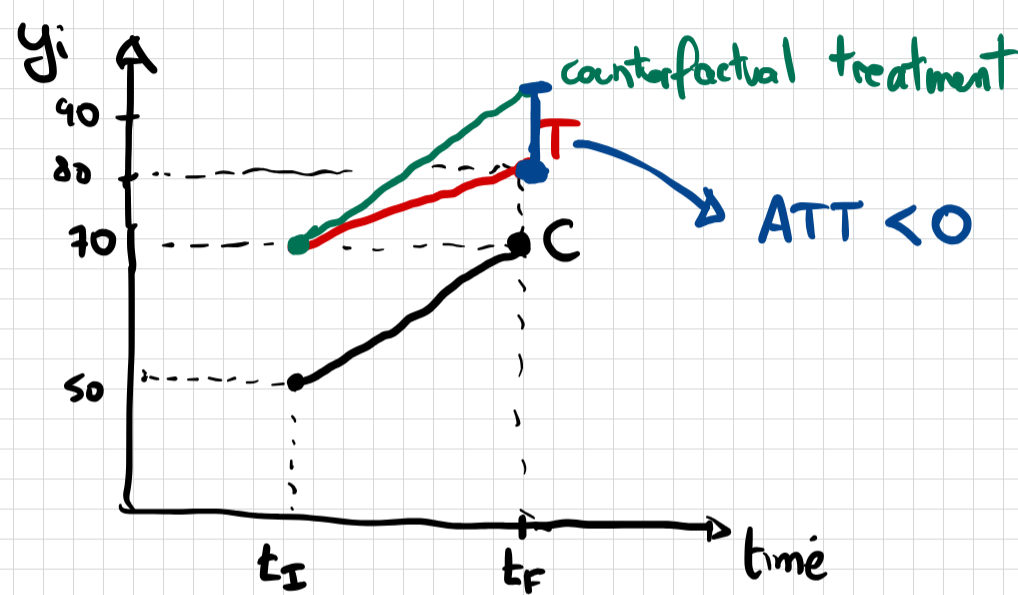
\includegraphics[width=0.5\linewidth]{Images/DiD.png}
    \caption{PTA Visualized}
\end{figure}
\end{rem}


\section{Commandments of Econometrics}
\fbox{
  \parbox{0.9\textwidth}{
    \textbf{(First Commandment)} Never assume homoskedasticity, always compute the robust 
    \[SE(\hat\beta)\]
    }}
Reason: almost never is, and hard to see!

\fbox{
  \parbox{0.9\textwidth}{
    \textbf{(Second Commandment)} Never build a model with perfect colinearity in $\textbf{X}.$
    }}
Reason: $\hat\beta$ won't exist!

    \fbox{
  \parbox{0.9\textwidth}{
    \textbf{(Third Commandment)} Never use OLS to estimate supply and demand. Use instrument variables instead. 
    }}
Reason: $P$ is endogenous!
\end{document}